% !TeX lualatex

%%%%%%%%%%%%%%%%%%%%%%%%%%%%%%%%
%% MUST COMPILE WITH LUALATEX %%
%%%%%%%%%%%%%%%%%%%%%%%%%%%%%%%%

\documentclass[oneside]{book}
\usepackage[a4paper]{geometry}
\geometry{textwidth=15.75cm, textheight=23.4cm, marginratio={4:6,5:7}}
\setlength{\parskip}{0.7\baselineskip} 

\usepackage{emoji}
\usepackage{hyperref}
\usepackage{cleveref}

\usepackage{soul}  % for the \hl command in snippets 
\usepackage{graphicx}

% table stuff
\usepackage{piton}
\usepackage{tabularray}
\UseTblrLibrary{tikz,diagbox,functional}
\usetikzlibrary{fadings}  % for the pqcrypto table
\usepackage{xcolor,luacolor}
\usepackage{tcolorbox}
\tcbuselibrary{breakable,skins}
\usepackage{lua-ul}
\LuaULSetHighLightColor{yellow!40}

\usepackage{adjustbox}  % for \adjustbox
\usepackage{changepage}  % for \adjustwidth
\usepackage{bbding}  % for \Checkmark and \XSolidBrush
\newcommand{\yes}{\textcolor{green!70!black}{\Checkmark}}
\newcommand{\no}{\textcolor{red!50}{\XSolidBrush}}

\usepackage{paralist}  % compactitem

\newtcolorbox{infobox}[1]{
    breakable,
    colback=green!15,
    colframe=green!65!black,
    fonttitle=\bfseries,
    title={#1},
    before skip balanced=\parskip,
    after skip balanced=\parskip,
    skin=enhanced,
}

\newtcolorbox{errorbox}[1]{
    breakable,
    colback=red!15,
    colframe=red!65!black,
    fonttitle=\bfseries,
    title={#1},
    before skip balanced=\parskip,
    after skip balanced=\parskip,
    skin=enhanced,
}

\newtcolorbox{questionbox}[1]{
    breakable,
    colback=violet!15,
    colframe=violet!65!black,
    fonttitle=\bfseries,
    title={#1},
    before skip balanced=\parskip,
    after skip balanced=\parskip,
    skin=enhanced,
}

\newtcolorbox{warningbox}[1]{
    breakable,
    colback=orange!15,
    colframe=orange!65!black,
    fonttitle=\bfseries,
    title={#1},
    before skip balanced=\parskip,
    after skip balanced=\parskip,
    skin=enhanced,
}

\newtcolorbox{standalonebox}{
    colback=white,
    hbox,
    colframe=white,
    left*=0mm,
    right*=0mm,
    bottom=0mm,
    top=0mm,
    boxsep=0mm,
    sharp corners,
    skin=enhanced,
}

% TODO find a way to avoid having to escape the special characters
\newcommand{\snippet}[1]{{\sethlcolor{gray!30}\hl{\texttt{#1}}}}


% Latex syntax highlighting with piton
\NewPitonLanguage{LaTeX}{keywordsprefix = \ , alsoother = @_ , moredirectives={&}, morecomment = [l]\%}
\PitonOptions{language = LaTeX, width=min, detected-commands = {highLight}, splittable=4}
\SetPitonStyle[LaTeX]{ Number = , Directive= \color{red!50}}

%%%%%%%%%%%
% Display the code, render it, and create a copy-pastable annotation on the right side
%%%%%%%%%%%

% Almost copy-pasted from https://github.com/fpantigny/nicematrix/blob/master/nicematrix.tex#L79
\ExplSyntaxOn
\dim_new:N \l__pantigny_width_dim
\bool_new:N \l__pantigny_show_output_bool
\bool_new:N \l__pantigny_small_bool
\bool_new:N \l__pantigny_execute_bool
\bool_new:N \l__pantigny_footnotesize_bool 

\keys_define:nn { pantigny }
  {
    width .dim_set:N = \l__pantigny_width_dim ,
    annotation .code:n = \PitonOptions { annotation = #1 } ,
    show-output .bool_set:N = \l__pantigny_show_output_bool ,
    show-output .default:n = true,
  }

\NewPitonEnvironment { Code } { O { } }
  {
    \begin{tcolorbox}[colback=blue!3, boxrule=0pt]
        \dim_zero:N \l__pantigny_width_dim
        \PitonOptions { annotation, indent-broken-lines, continuation-symbol=\empty, end-of-broken-line=\empty, continuation-symbol-on-indentation=\empty }
        \keys_set:nn { pantigny } { #1 }
        \group_begin:
        \char_set_catcode_other:N |
        \color{gray}

        \small
        \dim_compare:nNnT \l__pantigny_width_dim > \c_zero_dim 
          { 
            \PitonOptions { width = \l__pantigny_width_dim  } 
            \begin{minipage}[c]{\l__pantigny_width_dim} 
          }
    }
    {
        \dim_compare:nNnT \l__pantigny_width_dim > \c_zero_dim 
          { \end{minipage} }
        \group_end:
        \bool_if:NTF \l__pantigny_show_output_bool
          {
                % \smallskip
                \vspace{-0.5em}
                \begin{center}\begin{standalonebox}
                    \lua_now:n { tex.print(piton.get_last_code():explode(string.char(10)))}
                \end{standalonebox}
                \end{center}
          }
      	  {
      	  	 \vspace{-0.2em}
      	  }
        \end{tcolorbox}
    }
\ExplSyntaxOff

%%%%
% for drawing the table in appendix
%%%%

% Inspired from https://tex.stackexchange.com/a/750321/430417
\IgnoreSpacesOn

\tlNew \gTikzPercentagePathsTl


\prgNewFunction \colMaxValue {m} {  
	\fpSet \lTmpaFp {\fpEval {\cellGetText{2}{#1}}}
	\intStepOneInline {2} {\arabic{rowcount}} {
		\fpSet \lTmpaFp {\fpMathMax{\lTmpaFp}{\fpEval {\cellGetText{##1}{#1}}}}
	}
	\prgReturn {\fpUse\lTmpaFp}
}

\prgNewFunction \barPlotPaths {m} {
	\tlClear \gTikzPercentagePathsTl
	\fpSet \lTmpaFp {\colMaxValue{#1}}
	\intStepOneInline {2} {\arabic{rowcount}} {
		\fpSet \lTmpbFp {\fpEval{\cellGetText{##1}{#1}}}  
		\fpSet \lTmpcFp {\fpMathDiv {\lTmpbFp} {\lTmpaFp}}
		\tlPutRight \gTikzPercentagePathsTl {
			\evalWhole{
				(##1-#1.south~west) rectangle
				($(##1-#1.north~west)!{\fpUse \lTmpcFp}!(##1-#1.north~east)$)
			}
		}
	}
}
\IgnoreSpacesOff


\newcommand{\ManualTitle}{Learning \texttt{tabularray}}
\newcommand{\ManualSubtitle}{A beginner-friendly tutorial for modern and powerful \LaTeX\ tables}
\newcommand{\ManualAuthor}{melepe (mmelepe@gmail.com)}
\newcommand{\ManualVersion}{Version 1.1}
\newcommand{\CompilationDate}{\today}
\newcommand{\FrenchVersion}{\url{https://zestedesavoir.com/tutoriels/5029/les-tableaux-en-latex-avec-tabularray/}}
\newcommand{\LatestVersion}{\url{https://github.com/mmelepe/tabularray_tutorial/blob/master/latest.pdf}}
\newcommand{\ShortVersion}{\url{https://github.com/mmelepe/tabularray_tutorial/blob/master/latest_short.pdf}}

\begin{document}
	
\definecolor{tblblue}{HTML}{2563EB}
\definecolor{tblcyan}{HTML}{06B6D4}
\definecolor{tblgray}{HTML}{64748B}

% Background table styles
\tikzset{
	bgtable/.style={
		text opacity=0.65
	},
}


\newgeometry{
	left=0mm,
	right=0mm,
	top=0mm,
	bottom=0mm
}

\thispagestyle{empty}

\begin{tikzpicture}[remember picture,overlay]
	
	% ----------------------------------------------------------
	% Background
	% ----------------------------------------------------------
	\fill[tblblue!7] (current page.south west) rectangle (current page.north east);
	
	\fill[tblblue!5]
	(current page.south east)
	-- (current page.north east)
	-- ([xshift=-8cm,yshift=-7cm]current page.north east)
	-- cycle;
	
	% ----------------------------------------------------------
	% Background table 1
	% ----------------------------------------------------------
	\node[bgtable, rotate=7]
	at ([xshift=-6.0cm,yshift=6.0cm]current page.south east)
	{
		\begin{tblrtikzabove}
			% ----------------------------------------------------
			% Status dots
			% ----------------------------------------------------
			\fill[tblblue!52] (2-2.center) circle (2pt);
			\fill[tblblue!81] (3-2.center) circle (2pt);
			\fill[tblblue!94] (4-2.center) circle (2pt);
			\fill[tblblue!86] (5-2.center) circle (2pt);
			
			% ----------------------------------------------------
			% Percentage bars
			% ----------------------------------------------------
			\fill[tblblue!52, rounded corners=2pt] (2-3.south west) rectangle ($(2-3.north west)!0.52!(2-3.north east)$);
			\fill[tblblue!81, rounded corners=2pt] (3-3.south west) rectangle ($(3-3.north west)!0.81!(3-3.north east)$);
			\fill[tblblue!94, rounded corners=2pt] (4-3.south west) rectangle ($(4-3.north west)!0.94!(4-3.north east)$);
			\fill[tblblue!86, rounded corners=2pt] (5-3.south west) rectangle ($(5-3.north west)!0.86!(5-3.north east)$);
			
			% ----------------------------------------------------
			% Highlight best row
			% ----------------------------------------------------
			\draw[tblcyan, rounded corners=2pt]
			([xshift=-2pt,yshift=2pt]4-1.north west) rectangle ([xshift=2pt,yshift=-2pt]4-4.south east);
		\end{tblrtikzabove}
		
		\begin{tblr}{
			colspec={Q[l,1.5cm] Q[c,0.5cm] Q[l,2.3cm] Q[c]},
			row{1}={tblblue!30, font=\sffamily\bfseries\scriptsize},
			row{2-Z}={font=\sffamily\scriptsize},
			rowsep=5pt,
			hline{1,Z}={1pt,tblblue!50},
		}
			Year & & Attendance & City \\
			2023 & & 72\% & The Hague \\
			2024 & & 81\% & Ho Chi Minh City \\
			2025 & & \textbf{94\%} & Milano\\
			2026 & & 86\% & Córdoba
		\end{tblr}
	};
	
	% ----------------------------------------------------------
	% Background table 2
	% ----------------------------------------------------------
	\node[bgtable, rotate=-8]
	at ([xshift=-3.5cm,yshift=0.5cm]current page.east)
	{
		\begin{tblr}{
			colspec={Q[1.4cm]Q[1.8cm]Q[1.8cm]},
			rows={ht=0.5cm},
			cells={font=\sffamily\scriptsize},
			row{1}={tblcyan!30, font=\sffamily\bfseries\scriptsize},
			hline{1,2,Z}={tblcyan!25},
			vline{1,Z}={tblcyan!20}
		}
			Product & Category & Price \\
			\SetCell[r=2]{m} Widget A & Tools & 19.95 \\
			& Books & 29.50 \\
			Widget C & Software & 49.00 \\
			Widget D & Hardware & 12.75
		\end{tblr}
	};
	
	% ----------------------------------------------------------
	% Background table 3
	% ----------------------------------------------------------
	
	% TODO Seems that there is a bug somewhere because the styling of the last column is not working
	\node[bgtable, rotate=5]
	at ([xshift=3.5cm,yshift=-2.5cm]current page.north)
	{
		\begin{tblr}{
			colspec = {lcccc},
			cells = {font=\scriptsize\sffamily},
			cell{1}{3,5} = {c=2}{c},        
			hline{2} = {3-4}{leftpos=-1,rightpos=-1,endpos=true,dotted},
			hline{2} = {5-6}{leftpos=-1,rightpos=-1,endpos=true,dotted},
		}
			&& Women && Men & \\
			&& Score & Confidence & Score & Confidence \\ \hline
			\SetCell[r=3]{m}Geometry & trig5      & 8.2 & 0.91 & 7.8 & 0.88 \\
			& trig8      & 7.4 & 0.87 & 6.9 & 0.81 \\
			& vision      & 6.7 & 0.84 & 7.3 & 0.89 \\ \hline[dotted,endpos=true,leftpos=-1,rightpos=-1]
			\SetCell[r=2]{m} Other    & semtest    & 9.1 & 0.95 & 8.6 & 0.92 \\
			& align      & 5.9 & 0.76 & 6.5 & 0.80 \\ \hline
		\end{tblr}
	};
	
	% ----------------------------------------------------------
	% Background table 4
	% ----------------------------------------------------------
	\node[bgtable, rotate=-5]
	at ([xshift=3.5cm,yshift=8.5cm]current page.south west)
	{
		\begin{tblr}{
			colspec={Q[l,m]|ccc},
			column{1} = {2cm},
			row{1}={tblcyan!20, font=\sffamily\bfseries\scriptsize},
			row{even} = {gray!30},
			row{odd[3]} = {gray!5},
			cells={font=\sffamily\scriptsize},
			hline{1,2,Z},
			vline{1,Z},
		}
			Feature & Basic & Pro & Elite \\
			Private rooms & \Checkmark & \Checkmark & \Checkmark \\
			Customization & \Checkmark & \Checkmark & \Checkmark \\
			Software updates & -- & \Checkmark & \Checkmark \\
			Customer support & -- & \Checkmark & \Checkmark \\
			Advanced monitoring & -- & -- & \Checkmark
		\end{tblr}
	};
	
	
	% ----------------------------------------------------------
	% Central white panel
	% ----------------------------------------------------------
	\fill[white, fill opacity=0.6, rounded corners=8pt]
		([xshift=2cm,yshift=12cm]current page.south west)
		rectangle
		([xshift=-2cm,yshift=-3cm]current page.north east);
	
	
	% % ----------------------------------------------------------
	% % "MANUAL" label
	% % ----------------------------------------------------------
	% \node[
	%   anchor=west,
	%   font=\sffamily\bfseries\small,
	%   text=tblblue,
	% ]
	%   at ([xshift=3.0cm,yshift=-5.1cm]current page.north west)
	%   {Tutorial};
	
	% ----------------------------------------------------------
	% Main title
	% ----------------------------------------------------------
	\node[anchor=west, font=\sffamily\bfseries\Huge]
		at ([xshift=3cm,yshift=-6.5cm]current page.north west)
		{\ManualTitle};
	
	% ----------------------------------------------------------
	% Subtitle
	% ----------------------------------------------------------
	\node[anchor=north west, text=tblgray, font=\sffamily\LARGE, text width=11.5cm,	align=left]
		at ([xshift=3cm,yshift=-7.5cm]current page.north west)
		{\ManualSubtitle};
	
	
	% ----------------------------------------------------------
	% Author / version information
	% ----------------------------------------------------------
	\node[anchor=north west, font=\sffamily\small]
		at ([xshift=6cm,yshift=-11cm]current page.north west)
		{Author: \textbf{\ManualAuthor}};
	
	\node[anchor=north west, text=tblgray, font=\sffamily\small]
		at ([xshift=6cm,yshift=-11.5cm]current page.north west)
		{\ManualVersion\quad\textbullet\quad Compiled \CompilationDate};
	
	\node[anchor=south east, text=tblgray, font=\sffamily\footnotesize, text width=11.7cm, align=right]
		at ([xshift=-1cm,yshift=0.5cm]current page.south east)
		{\textbf{WTFPL 2}\\[2pt] This document is licensed under the Do What The Fuck You Want Public License 2.};
	
	\node[anchor=south west, text=tblgray, font=\sffamily\footnotesize, align=left]
		at ([xshift=2.5cm,yshift=12cm] current page.south west)
		{
			Lastest version on Github: \LatestVersion \\
			French version: \FrenchVersion
		};
\end{tikzpicture}

\restoregeometry


\chapter*{Introduction}
\LaTeX is a very powerful typesetting language, that allows you to create PDFs of great aesthetic quality. However, not everything in that language is easy to learn, and tables are no exception. 

Latex veterans know that creating a table ever so slightly complicated usually requires several conflicting packages, multiple pilgrimages to StackExchange and numerous desperate dark magic incantations in the hope of getting a satisfying result.

Luckily, in 2021 a new package, tabularray\footnote{\url{https://ctan.org/pkg/tabularray}}, was created. It is a modern table setting library, which unified several existing techniques and functionalities, along with an emphasis on simplicity of use\footnote{Another package, \texttt{nicematrix}, also offers powerful and resilient table formatting. Its main advantage over tabularray is its integration in math environments and some specific advanced functionalities, its main disadvantage is its inability to break a table on several pages and impossibility to separate the styling from the data like in tabularray. I do not think there exists a beginner's tutorial for nicematrix, but you can have a look at the official documentation: \url{https://mirrors.ctan.org/macros/latex/contrib/nicematrix/nicematrix.pdf}.}.

\begin{infobox}{Target audience}
This non-official tutorial is aimed at anyone who knows the bases of Latex (how to create a basic "hello world" document is enough), and is interested into learning how to create tables. No prior experience with tables in Latex is required.

If you are already familiar with Latex tables, or if you are in a hurry, you can directly skip to the summary at the end of each section.

A short version of this tutorial is also available at \ShortVersion.
\end{infobox}

The first part of the tutorial give teach you the fundamentals for writing tables, especially with tabularray. This will be more than enough for 99\% of the tables you will ever create. In the case where more advanced tables are necessary, the second part of this tutorial will guide you step by step.

Finally, an appendix completes the tutorial, with extra details, a FAQ, and the solution to the exercises.

\tableofcontents


\part{Simple tables without hassle}

\chapter{Creating a basic table}\label{sec:basic}

\section{Your first tabularray table}
Let's start from the beginning, with a simple example that we will be able to analyse in detail. 
In order to use tabularray in your Latex file, you simply have to include the package in the document preamble. 

\begin{Code}
\documentclass{article}  % or any other documentclass
\usepackage{tabularray}

\begin{document}
  % Your tabularray table here
\end{document}
\end{Code}

The example below shows a minimal table example, with 2 rows and 3 columns, and centered text in each cell:

% TODO use a tcblisting for having the \begin{document} in the first snippet?
\begin{Code}[show-output]
\begin{tblr}{ccc}
	Hello & tabularray & world! \\
	cell & other cell & last cell \\
\end{tblr}
\end{Code}

\begin{warningbox}{Compilation error?}
If the above example does not compile on your machine, it is probable that your Latex distribution is not up to date or that tabularray is not installed. Please refer to the FAQ in \Cref{app:version} to update your distribution.

Moreover, many examples and functionalities in this tutorial rely on the 2025A version. All examples might not work with your current tabularray version, please refer to \Cref{app:version} in case of doubt.
\end{warningbox}

For the moment, our table is ugly, but that's a problem for later \emoji{smiley}. Let's analyze our code piece by piece:

\begin{itemize}
    \item \snippet{\textbackslash begin\{tblr\}} and \snippet{\textbackslash end\{tblr\}} indicate the beggining and the end of the table, respectively.
    \item Columns are specified directly after the \snippet{\textbackslash begin\{tblr\}}, between two curly braces \snippet{\{\}}. Here, we want three columns with horizontally centered text (type \snippet{c}, we will see other types later on), which gives us \snippet{\{ccc\}}.
    \item Table data itself. You just have to write the contents of our table, using the following two formatting tools:
    \begin{itemize}
        \item \snippet{\&} for separating successive cells in the same row;
        \item \snippet{\textbackslash\textbackslash} to indicate the end of the row.
    \end{itemize}
\end{itemize}

A cell can contain any kind of text, images, mathematical code, and many other things, or even nothing at all. The two things to remember are that a cell is separated from the next cell by the ampersand \snippet{\&} and that you must ensure there is the correct number of cells in a row (otherwise, the result might be unexpected).

\begin{questionbox}{}
What if I want to use \snippet{\&} or \snippet{\textbackslash\textbackslash} in my table?
\end{questionbox}

That is very much feasible, you just have to escape the characters, as usual in Latex:

\begin{Code}[show-output]
\begin{tblr}{cc}
	\&                           & cell separator \\
	\textbackslash\textbackslash & row separator \\
\end{tblr}
\end{Code}

Note that in this code snippet, the ampersands were aligned so that the table structure was directly visible in the Latex source code. This is not mandatory and changes nothing to the final rendered table (surrounding spaces are ignored by Latex as a general rule), but it's more practical when you are editing your table. It is a good habit to catch!

You obviously can create a table with any number of rows and columns. The only important thing is to specify the correct number of columns just after \snippet{\textbackslash begin\{tblr\}} and to use \snippet{\textbackslash\textbackslash} to indicate the next row.

For instance, the code below will give the expected result (but definitely not a balanced diet):

\begin{Code}[show-output]
\begin{tblr}{cccccccc}  % 8 centered columns
	       & Monday   & Tuesday  & Wednesday & Thursaday & Friday   & Saturday & Sunday \\
	Lunch  & Potatoes & Potatoes & Potatoes  & Potatoes  & Potatoes & Potatoes & Potatoes too! \\ 
	Dinner & Rice     & Stir-fry & Soup      & Eat out   & Fish     & Pizza    & Leftovers \\
\end{tblr}
\end{Code}

Note that the first cell is empty, that's why there is no text before the first \snippet{\&}. But you \emph{must} keep the \snippet{\&} in the code, otherwise everything would be shifted (give it a try).

\section{Column alignment}

Until now, we always used horizontally centered columns. But there are other column types!

\begin{itemize}
\item columns of type \textbf{c}, which will \textbf{c}enter the text
\item columns of type \textbf{l}, which will align the text to the \textbf{l}eft
\item columns of type \textbf{r}, which will align the text to the \textbf{r}ight
\item columns of type \textbf{j}, which will \textbf{j}ustify the text in multiline cells (we will see how to do that later).
\end{itemize}

%You can combine several kinds of columns in the same table.

\begin{Code}[show-output]
\begin{tblr}{rlcc}  % 1 right align, 1 left, 2 center
	Surname       & Name           & Grade   & Comment \\
	Jean-Pierre   & Dupuis         & 13/20   & Good progress this semester.\\
	Marie         & Pranel--Mathon & 11/20   & You need to work more! \\
	Brahim        & Sarou          & 15/20   & Very good work, congrats! \\
\end{tblr}
\end{Code}

\section{Adding horizontal and vertical borders}
Until now, our tables are hopelessly ugly \emoji{frowning-face}, notably becayse we are not yet using any borders. 
Fortunately, vertical and horizontal borders are very easy to add to your table! 

\begin{itemize}
\item For horizontal borders, you need to write \snippet{\textbackslash hline} at the row where you want the border (before the row for a border above, after the row for a border below)
\item For vertical borders, they can be defined within the column specification. For instance, instead of writing \snippet{\{rlcc\}}, one can write \snippet{\{|rl|cc|\}}, where each vertical pipe \snippet{|} indicates a vertical border. Thus, the colspec \snippet{\{|rl|cc|\}} will create a vertical border before the first column, between the second and third columns, and after the fourth column.
\end{itemize}

\begin{Code}[show-output]
\begin{tblr}\highLight{{|rl|cc|}}  % some vertical borders
	\highLight{\hline}  % horizontal border before the first row
	Surname       & Name           & Grade   & Comment \\ 
	\highLight{\hline}  % another
	Jean-Pierre   & Dupuis         & 13/20   & Good progress this semester.\\
	Marie         & Pranel--Mathon & 11/20   & You need to work more! \\
	Brahim        & Sarou          & 15/20   & Very good work, congrats! \\
	\highLight{\hline}  % a last border
\end{tblr}
\end{Code}

Of course, you can add borders wherever you want, and as many as you want. You can even use double, triple or even more borders, even though it becomes quickly unreadable.

%
%\begin{Code}[show-output]
%\begin{tblr}\highLight{{|rl||cc|}}  % double border
%	\hline
%	Surname       & Name           & Grade   & Comment \\ 
%	\hline
%	Jean-Pierre   & Dupuis         & 13/20   & Good progress this semester.\\
%	Marie         & Pranel--Mathon & 11/20   & You need to work more! \\
%	Brahim        & Sarou          & 15/20   & Very good work, congrats! \\
%	\hline
%\end{tblr}
%\end{Code}

\begin{warningbox}{Love is without borders}
Do not overuse borders! A clean, uncluttered table is much easier to read than one with borders everywhere. To give you an example, what do you prefer between 

\begin{center}
\begin{standalonebox}
\begin{tblr}{colspec={|rl||cc|}, hlines, vlines}   
	Surname       & Name           & Grade   & Comment \\ 
	\hline
	Jean-Pierre   & Dupuis         & 13/20   & Good progress this semester.\\
	Marie         & Pranel--Mathon & 11/20   & You need to work more! \\
	Brahim        & Sarou          & 15/20   & Very good work, congrats! \\
\end{tblr}
\end{standalonebox}
\end{center}

and

\begin{center}
\begin{standalonebox}
\begin{tblr}{colspec={rlcc}}   
	Surname       & Name           & Grade   & Comment \\ 
	\hline
	Jean-Pierre   & Dupuis         & 13/20   & Good progress this semester.\\
	Marie         & Pranel--Mathon & 11/20   & You need to work more! \\
	Brahim        & Sarou          & 15/20   & Very good work, congrats! \\
\end{tblr}
\end{standalonebox}
\end{center}

It is up to you to decide how many borders are too many. General recommandations are: 

\begin{itemize}
\item Do not use double borders
\item Avoid vertical borders as much as possible\footnote{There are people who find vertical borders unprofessional. I would not go this far, but I do agree that most of vertical borders are useless anyways.}
\item Limit the number of borders, usually three horizontal lines (before the first row, after the first row, and after the last row) are enough
\item Left alignment is often a good idea.
\end{itemize}

More information in the folllowing guide: \url{https://people.inf.ethz.ch/markusp/teaching/guides/guide-tables.pdf}. In this tutorial, we will use a lot of vertical borders, but mostly because they are useful to show where a cell ends. In general, it is better to stick with the rule of no vertical border.
\end{warningbox}

\section{Compatibility with native Latex tables}
In this tutorial, we will only deal with tabularray tables. But many people still use native Latex tables. Good news: everything we saw until here is also valid for native Latex tables (except the \snippet{j} column type). The only difference is that native tables use the environment \snippet{\textbackslash begin\{tabular\}} and \snippet{\textbackslash end\{tabular\}} rather than \snippet{tblr}, and do not require to load any external library.

Now, the same code will produce a more pleasant table in tabularray, and all the functionalities we will see afterwards are much easier to invoke in tabularray than in native tables and the army of packages we would need otherwise.

Let us have a comparison between a native and a tabularray table:

\begin{Code}[show-output]
\begin{tabular}{ccc}
	Owner   & Floor & Portion \\
	\hline
	Dumont  & 0     & $\frac{150}{1000}$ \\
	Gosso   & 1     & $\frac{200}{1000}$ \\
	Carrier & 1     & $\frac{150}{1000}$ \\
	Dumont  & 2     & $\frac{300}{1000}$ \\
	Montrin & 3     & $\frac{200}{1000}$ \\
\end{tabular}

\hspace{1em}  % horizontal separation

\begin{tblr}{ccc}
	Owner   & Floor & Portion \\
	\hline
	Dumont  & 0     & $\frac{150}{1000}$ \\
	Gosso   & 1     & $\frac{200}{1000}$ \\
	Carrier & 1     & $\frac{150}{1000}$ \\
	Dumont  & 2     & $\frac{300}{1000}$ \\
	Montrin & 3     & $\frac{200}{1000}$ \\
\end{tblr}
\end{Code}

You’ll appreciate tabularray straight away \emoji{grinning}. In the rest of this tutorial, we will look at commands that are specific to tabularray and which are no longer compatible with Latex’s native tables.

\begin{infobox}{TL;DR}
\begin{itemize}
    \item A tabularray table is similar to native Latex tables, and is declared with the \snippet{\textbackslash begin\{tblr\}} and \snippet{\textbackslash end\{tblr\}} environment (do not forget to add \snippet{\textbackslash usepackage\{tabularray\}} in the preamble!).
    \item You must specify the type of each column (\snippet{l}, \snippet{c}, \snippet{r} or \snippet{j}) and separate each cell by \snippet{\&}, and each row by \snippet{\textbackslash\textbackslash}.
    \item Horizontal borders are specified with \snippet{\textbackslash hline}. Vertical borders are added in the colspec with pipes \snippet{|}, for instance the colspec \snippet{c|lr} will add a vertical border between the \snippet{c} and \snippet{l} columns.
\end{itemize}

\textbf{\underline{Exercise}}: can you recreate the following table? Pay attention to the columns alignment.
\begin{center}
\begin{standalonebox}
\begin{tblr}{|l|c|r|}
   \hline
   Hello & tabularray  & world! \\
   cell  & cell & last table cell \\
   \hline
\end{tblr}
\end{standalonebox}
\end{center}

The solution is in \Cref{app:solution_basic}
\end{infobox}
\chapter{Control the cells and columns}\label{sec:control}

We saw that there were 4 types of columns. Actually, I lied: there is only one type of column! It's the column \snippet{Q}. This column can receive a ton of optional parameters (between square brackets \snippet{[]}). For instance:

\begin{itemize}
	\item \snippet{Q[l]} is a left-aligned column
	\item \snippet{Q[c]} is a centered column
	\item \snippet{Q[r]} is a right-aligned column
	\item \snippet{Q[j]} is a justified column
\end{itemize}

By default, \snippet{Q} (without any option) is a justified column, and thus is equivalent to \snippet{Q[j]}.

\begin{infobox}{}
	The columns \snippet{l}, \snippet{c}, \snippet{r}, \snippet{j} that we saw in the previous chapter are aliases of \snippet{Q[l]}, \snippet{Q[c]}, \snippet{Q[r]}, \snippet{Q[j]}, respectively.
\end{infobox}

You'll ask me what's the point? The idea of keeping the \snippet{l}, \snippet{c}, \snippet{r}, \snippet{j} is retro-compatibility with native Latex table (it's also faster to type and easier for a human to parse). The idea of the \snippet{Q} syntax is that we can also pass it numerous other options, that we will see just now.

\section{Control column width}

First of all, if you experimented a bit on your own, you might have noticed that the width of a column depends on its contents: if one cell is very large, then its column will be very large. In extreme cases, your table will overflow!

\begin{Code}[show-output]
\begin{tblr}{|l|l|l|}
	Pseudo & Comment & Date \\ \hline
	melepe & Amazing! & Yesterday\\
\end{tblr}
\end{Code}
\begin{Code}[show-output]
\begin{tblr}{|l|l|l|}
	Pseudo & Comment & Date \\ \hline
	melepe & Amazing! & Yesterday \\
	melepe & Ah also I wanted to give a huge shoutout to my friends, to my family and my team who have always been there for me & Today \\
\end{tblr}
\end{Code}

On one hand, it's practical when your text has a reasonable length, because you don't have to compute the column width on your own. On the other hand, you cannot have long text in such tables. 

Instead, tabularray offers the possibility to specify a column width: in centimeters (\snippet{cm}), points (\snippet{pt}), or any other Latex measuring unit (see \url{https://en.wikibooks.org/wiki/LaTeX/Lengths}). You don't know which one to chose? Keep it simple and use centimeters.

To define a column width, simply write it in the column's options. For instance, \snippet{Q[4cm]} defines a 4cm wide column. We can of course mix horizontal alignment options too, for instance \snippet{Q[l, 4cm]}. 
Let's see it in action:

\begin{Code}[show-output]
\begin{tblr}{|l|Q[l]|l|}  % Same table as previously, but we use a Q[l]
	Pseudo & Comment & Date \\	\hline
	melepe & Amazing! & Yesterday\\
\end{tblr}
\end{Code}
\begin{Code}[show-output]
\begin{tblr}{|l|\highLight{Q[l,4cm]}|l|}  % Column will be 4cm even if the text is too short
	Pseudo & Comment & Date \\ \hline
	melepe & Amazing! & Yesterday\\
\end{tblr}
\end{Code}
\begin{Code}[show-output]
\begin{tblr}{|l|\highLight{Q[l,4cm]}|l|}  % Column will be 4cm even if the text is too long
	Pseudo & Comment & Date \\ \hline
	melepe & Amazing! & Yesterday \\
	melepe & Ah also I wanted to give a huge shoutout to my friends, to my family and my team who have always been there for me & Today \\
\end{tblr}
\end{Code}

Now you know in which context the \snippet{j} column can be relevant.

\section{Control column vertical alignment}

Now that we have multiline cells, we must take into account vertical alignment. In the examples above, we see that the text is aligned at the top of the cells. 

Let's start with two placement options: 

\begin{itemize}
	\item At the top of the cell, with the option \snippet{h} (for \textbf{h}ead)
	\item At the end of the cell, with the option \snippet{f} (for \textbf{f}oot)
\end{itemize}

This option must be passed as an argument to the column \snippet{Q}. It can of course be cumulated with the options we saw before.

\begin{Code}[show-output]
\begin{tblr}{|\highLight{Q[f,l]}|Q[4cm]|l|} 
	% No horizontal alignment given for the second column so the default option (j) applies.
	Pseudo & Comment & Date \\
	\hline
	melepe & Amazing! & Yesterday \\
	melepe & Ah also I wanted to give a huge shoutout to my friends, to my family and my team who have always been there for me & Today \\
\end{tblr}
\end{Code}

The default value for vertical alignment is... neither of these two values \emoji{grinning}. By default, text is aligned on what we call the \emph{baseline}.

There are three possible placements of the baseline:

\begin{itemize}
	\item Under the first line of the text block, using the \textbf{t} option (\textbf{t}op). This is the default option
	\item Under the last line of the text block, using the \textbf{b} option (\textbf{b}ottom)
	\item In the \textbf{m}iddle between the top and bottom lines, using the \textbf{m} option 
\end{itemize}

\begin{Code}
\begin{tblr}{|l|\highLight{Q[b,4cm]}|l|}
	Pseudo & Comment & Date \\
	\hline
	melepe & Amazing! & Yesterday \\
	melepe & Ah also I wanted to give a huge shoutout to my friends, to my family and my team who have always been there for me & Today \\
\end{tblr}
\end{Code}

Will render like so (I added the baseline in red):
\begin{center}
\begin{standalonebox}
% base anchor is at the baseline level
\begin{tblrtikzabove}
	\draw[red, dashed, thick] (3-1.base west) -- (3-3.base east);
\end{tblrtikzabove}

\begin{tblr}{|l|Q[b,4cm]|l|}
	Pseudo & Comment & Date \\
	\hline
	melepe & Amazing! & Yesterday \\
	melepe & Ah also I wanted to give a huge shoutout to my friends, to my family and my team who have always been there for me & Today \\
\end{tblr}
\end{standalonebox}
\end{center}

It's so simple, and yet, compared to the hell you need to go through to get the same result with native Latex tables, it's a revolution!

\begin{warningbox}{Baseline alignment is not text alignment}
	Be careful, as we said the vertical alignment will align the \emph{baseline}, not the text itself. This will give counter-intuitive results when several cells are multiline.
	
\begin{Code}
\begin{tblr}{|Q[2cm,b]|Q[2cm,t]|Q[2cm,m]|}
\hline
baseline set to b & baseline set to t & baseline set to m \\
\hline
\end{tblr}
\end{Code}
Will render as so (I added the baseline in red):

\begin{center}
\begin{standalonebox}
\begin{tblrtikzabove}
	\draw[red, dashed, thick] (1-1.base west) -- (1-3.base east);
\end{tblrtikzabove}
\begin{tblr}{|Q[2cm,b]|Q[2cm,t]|Q[2cm,m]|}
	\hline
	baseline set to b & baseline set to t & baseline set to m \\
	\hline
\end{tblr}
\end{standalonebox}
\end{center}
\end{warningbox}

Combining every possible option into one table, we get the following result.

\begin{Code}[show-output]
\begin{tblr}{|Q[2cm,b]|Q[2cm,t]|Q[2cm,m]|Q[2cm,m]|Q[2cm,h]|Q[2cm,f]|}
	\hline
	baseline set to b & baseline set to t & baseline set to m with a lot of text that is going on forever & baseline set to m & placement with h & placement with f\\ \hline
\end{tblr}
\end{Code}

Note that options \snippet{h} and \snippet{b} are not equivalent, and neither are \snippet{f} and \snippet{t}.

\section{Multiline cells}
Sometimes, it is useful to write several lines in a cell, and deciding yourself where you want the line break. For this, there is a very simple solution: put the cell text in-between curly braces \snippet{\{\}}, and now you are able to use the Latex command for linebreak: \snippet{\textbackslash\textbackslash}. 

\begin{Code}[show-output]
	\begin{tblr}{lll}
		Country    & Capital(s)             & Comment \\ \hline
		Belize     & Belmopan                & N/A \\
		Bénin      & \highLight{{Porto-Novo \\ Cotonou}} & \highLight{{Official capital \\ De facto administrative capital}}\\
		Bhutan & Thimphu                 & N/A \\
	\end{tblr}
\end{Code}

Of course, multiline cells can be horizontally or vertically aligned. In the following example, observe how ``Bénin'' is now vertically centered with the rest of the row.

\begin{Code}[show-output]
	\begin{tblr}\highLight{{lQ[l,m]Q[l,m]}}
		Country    & Capital(s)             & Comment \\ \hline
		Belize     & Belmopan                & N/A \\
		Bénin      & {Porto-Novo \\ Cotonou} & {Official capital \\ De facto administrative capital}\\
		Bhutan & Thimphu                 & N/A \\
	\end{tblr}
\end{Code}

\section{Columns spanning all the available space}

tabularray also has another column, the column \snippet{X}\footnote{This column is also an alias of the column \snippet{Q}, more specifically is an alias of \snippet{Q[co=1]}. But it's often easier to use the \snippet{X} notation, in resemblance to tabularx package. The \snippet{X} column notation also accepts optional arguments, e.g. \snippet{X[l,m]}.}. An \snippet{X} column will calculate the remaining free space available across the page width, and automatically fill this space. If there are several \snippet{X} columns in the table, the space is equally distributed over these columns, meaning they will all have the same width.

\begin{Code}[show-output]
% Reference table
\begin{tblr}{ll|l|l|}
	Furniture & Price & Shop     & Comment \\ \hline
	Bed       & 150   & MOBILI   & An entry-level, without mattress. \\
	Table     & 800   & LUXTABLE & We'll be able to impress our guests \\
	Desk      & 300   & LBC      & Essential for remote work \\
\end{tblr}
\end{Code}
\begin{Code}[show-output]
\begin{tblr}\highLight{{ll|X|X|}}
	Furniture & Price & Shop     & Comment \\ \hline
	Bed       & 150   & MOBILI   & An entry-level, without mattress. \\
	Table     & 800   & LUXTABLE & We'll be able to impress our guests \\
	Desk      & 300   & LBC      & Essential for remote work \\
\end{tblr}
\end{Code}

If you don't want the table to span over the whole page width, but still want to use  \snippet{X} columns, you just have the specify the desired total width in the table header and tabularray will manage. Small but important detail, now that there are several arguments in the header (the column specification and the table width), the colspec must be specified using the keyword \snippet{colspec=\{...\}}.

\begin{Code}[show-output]
\begin{tblr}{
	\highLight{width=0.7\linewidth,}  % 70 % of maximum line width. One can also input a value in cm, pt or whatever.
	colspec={ll|X|X|},
}
	Furniture & Price & Shop     & Comment \\ \hline
	Bed       & 150   & MOBILI   & An entry-level, without mattress. \\
	Table     & 800   & LUXTABLE & We'll be able to impress our guests \\
	Desk      & 300   & LBC      & Essential for remote work \\
\end{tblr}
\end{Code}

\begin{errorbox}{Blank lines and tabularray}
There cannot be blank lines in a tabularray header, it would break compilation. For instance, the following table will generate a compilation error:

\begin{Code}
\begin{tblr}{
	width=0.7\linewidth,
\highLight{                                                 }	
	colspec={ll|X|X|},
}
	Furniture & Price & Shop     & Comment \\ \hline
	Bed       & 150   & MOBILI   & An entry-level, without mattress. \\
	Table     & 800   & LUXTABLE & We'll be able to impress our guests \\
	Desk      & 300   & LBC      & Essential for remote work \\
\end{tblr}
\end{Code}

Similarly, too many blank lines in the body of the table might cause unexpected issues. In the example below, the code compiles, but the cell ``Table'' is not correctly aligned:

\begin{Code}[show-output]
\begin{tblr}{
		width=0.7\linewidth,
		colspec={llXX},
}
	Furniture & Price & Shop     & Comment \\ \hline
	Bed       & 150   & MOBILI   & An entry-level, without mattress. \\
	% Empty lines
\highLight{                                                }
\highLight{                                                }
\highLight{                                                }
	Table     & 800   & LUXTABLE & We'll be able to impress our guests \\
	Desk      & 300   & LBC      & Essential for remote work \\
\end{tblr}
\end{Code}

tabularray does not guarantee correct results if there are two or more consecutive blank lines. However, lines with only a comment do not count as blank lines.
\end{errorbox}

For a finer setting of the column size, it is possible to give an argument to the \snippet{X} column. This argument is a priority coefficient, for when there are several \snippet{X} columns in the table. Remember that, by default, the remaining space is distributed equally. Thanks to this coefficent, it is possible to adjust this distribution.

For instance, \snippet{X[2]} is a column that has a coefficient of 2, \snippet{X[3]} has coefficient 3, and so on. By default, \snippet{X} is equivalent to \snippet{X[1]}.

\begin{Code}[show-output]
\begin{tblr}\highLight{{ll|X|X[2]|}}
	Furniture & Price & Shop     & Comment \\ \hline
	Bed       & 150   & MOBILI   & An entry-level, without mattress. \\
	Table     & 800   & LUXTABLE & We'll be able to impress our guests \\
	Desk      & 300   & LBC      & Essential for remote work \\
\end{tblr}
\end{Code}

Finally, note that \snippet{X} can receive other options, such as horizontal alignment (\snippet{l}, \snippet{c}, \snippet{r}, \snippet{j}), or vertical alignment (\snippet{t}, \snippet{f}...): \snippet{X[3,m,j]} is a valid column.


\section{Merged cells}
Another highly appreciated functionality of tabularray if the ability to merge cells with ease. Let's look at the following table:

\begin{Code}
\begin{tblr}{l|l|l}
		  & Monday     & Tuesday \\ \hline
	8:00  & Literature & History \\ \hline
	9:00  & Math       & PE \\ \hline
	10:00 & Math       & Literature \\ \hline
	11:00 & History    & Biology \\ \hline
\end{tblr}
\end{Code}

It could be interesting to merge the Monday 9:00 and 10:00 cells, since it is the same class. 
We can use the command \snippet{\textbackslash SetCell} to do so. Let's first show how to use it in our example:

\begin{Code}[show-output]
\begin{tblr}{l|l|l}
		  & Monday     & Tuesday \\ \hline
	8:00  & Literature & History \\ \hline
	9:00  & \highLight{\SetCell[r=2]{l,m} Math      } & PE \\ \hline
	10:00 & \highLight{      } & Literature \\ \hline
	11:00 & History    & Biology \\ \hline
\end{tblr}
\end{Code}

Note that the horizontal line automatically disappeared between the merged cells. Also note that the cell that is ``overwritten'' by the merged cell must still be indicated with a \snippet{\&}, even though it will not be displayed. Its content is irrelevant, as it will be overwritten by the contents of the cell containing the \snippet{\textbackslash SetCell}\footnote{This can lead to frustrating debugging sessions: the text you are writing is not appearing in the table, and you finally realize that you are writing text in a merged cell that is overwritten and therefore the text will never be displayed \emoji{poop}.}.

Let us now explain the \snippet{\textbackslash SetCell} command. It takes an optional argument and a mandatory one:

\begin{itemize}
	\item \snippet{[r=2]} indicates that we will merge 2 \textbf{r}ows together, starting from the cell we are.
	\item \snippet{\{l,m\}} indicates the horizontal and vertical alignment of the merged cell. Here, we used \snippet{l,m} so the cell will be left aligned, vertically centered. You had that right? If not, read the chapters on horizontal and vertical alignment again \emoji{slightly-smiling-face}. As a general rule, we can pass to the mandatory argument (in curly braces \snippet{\{\}}) of \snippet{\textbackslash SetCell} any option we could pass to a cell: width, alignment... We can also leave the curly braces empty if we don't want to specify anything.
\end{itemize}

We can also merge columns together, with the optional argument \snippet{[r=4]} (here, merging 4 columns). Finally, one can merge both rows and columns together:

\begin{Code}[show-output]
\begin{tblr}{|l|l|l|l|l|}
	\hline
	1 & 2                                & 3 & \highLight{\SetCell[c=2]{c}} 4,5 & not displayed!\\ \hline
	1 & \highLight{\SetCell[r=2,c=3]{r,m,4cm}} 2,3,4 & 0 & 0                    & 5 \\ \hline
	\highLight{\SetCell[r=2]{}} 1 &                  &   &                      & 5 \\ \hline
	& 2                                  & 3 & 4                    & 5 \\ \hline
\end{tblr}
\end{Code}


\begin{infobox}{TL;DR}
	\begin{itemize}
		\item Every column is actually a \snippet{Q} type column: \snippet{Q[l]}, \snippet{Q[c]}, \snippet{Q[r]} or \snippet{Q[j]}.
		\item Columns can be given a width: \snippet{Q[l, 5cm]}. Cells can also be given a width: \snippet{\textbackslash SetCell\{5cm\}}.
		\item Baseline alignment is done with the options \snippet{t}, \snippet{m}, \snippet{b} (for example, \snippet{Q[l,m,3cm]}). You can also use the options \snippet{h}, \snippet{f} to respectively position the text at the head (top) or the foot (bottom) of the cell.
		\item Columns of type \snippet{X} fill all the available space. Their size can be adjusted as follows: \snippet{X[2]}. It can receive other arguments: \snippet{X[2,c,m]}.
		\item Cells are merged with the example command \snippet{\textbackslash SetCell[r=2,c=3]\{l,m\}}, or similar. \snippet{r=} counts the number of merged \textbf{r}ows, \snippet{c=} counts the number of merged \textbf{c}olumns. Here, on top of that, \snippet{l,m} give the merged cell's alignment (left and vertically centered). We can leave the \snippet{\{\}} empty, or conversely write any styling instruction a cell can receive. The text from overwritten cells is not displayed (except the cell containing the \snippet{\textbackslash SetCell}).
		\item \snippet{\{Multiline \textbackslash\textbackslash~ cell\}} is a multiline cell.
	\end{itemize}

\textbf{\underline{Exercise}}: recreate this table.
\begin{center}
\begin{standalonebox}
\begin{tblr}{
		colspec={Q[1.5cm]lXX[2,j]},
		width=0.8\linewidth,
	}
	\SetCell[c=2]{c} Region &             & Celebrity                                        & Short bio \\ \hline
	\SetCell[r=3]{m} Europe & Russia      & \SetCell[r=2]{} {Leonhard Euler \\(1707--1783) } & \SetCell[r=2]{}   One of the greatest mathematicians in history, he also made significant contributions to mechanics, fluid dynamics, optics and astronomy.\\  \hline
	empty                   & Switzerland & empty                                            & not displayed either \\ \hline
							& Greece  & {Socrates \\(-470 -- -399)}                          & One of the founders of philosophy. He left no written works; the only record of his thinking comes from his pupils Plato and Xenophon. \\ \hline
	\SetCell[r=2]{} Asia    & Japan       & {Katsushika Hokusai \\(1760--1849)}              & A painter, draughtsman and printmaker, he is world-renowned for his woodblock print \textit{The Great Wave off Kanagawa}. He had a lasting influence not only on Japanese art, but also on European art (Van Gogh, Monet, Degas, etc.) \\ \hline
							& India       & {Suśruta \\ (around -600)}                       & He wrote one of the seminal texts on Ayurvedic medicine and made major discoveries in the fields of cataract surgery and plastic surgery. He is regarded as the father of surgery. \\ \hline
\end{tblr}
\end{standalonebox}
\end{center}

The table must have a width of \snippet{0.8\textbackslash linewidth}, the first column must measure 1.5cm, and the last two columns must be \snippet{X} columns (note that they do not have the same width).

The solution is available in \Cref{app:solution_control}.
\end{infobox}

\vfill 

\begin{infobox}{End of the first part}
	You now know enough about tabularray to create 99\% of the tables you will ever need to create. You can stop here for your first read-through. Experiment a bit, create your own tables, and when you will feel like it, come back and learn more with the next chapters!
	\vspace{1em}
	
	By the way, if creating the tables by hand is too tedious, you can also use the website \url{https://www.latex-tables.com/}. You can generate tabularray tables by selecting ``tabularray'' in the ``Latex environment'' dropdown.
\end{infobox}

\vfill

\part{More hassle with less simple tables}
\chapter{Manage separations and spacing}\label{sec:separations}

The previous chapter covered cell and column management. We will now deal with how our cells and columns are separated. This chapter will be brief, enjoy it while it lasts \emoji{grinning}.

\section{Add all separation lines}
If you want to display all horizontal and/or vertical lines, there is a command for that. Since the option is passed to tabularray's header, do not forget to put the colspec inside the keyword argument \snippet{colspec=\{...\}}.

\begin{Code}[show-output]
\begin{tblr}{
	\highLight{hlines},  % displays all horizontal lines
	\highLight{vlines},  % displays all vertical lines
	colspec = {cccccccc},
}
	& Monday   & Tuesday  & Wednesday & Thursaday & Friday   & Saturday & Sunday \\
	Lunch  & Potatoes & Potatoes & Potatoes  & Potatoes  & Potatoes & Potatoes & Potatoes too! \\ 
	Dinner & Rice     & Stir-fry & Soup      & Eat out   & Fish     & Pizza    & Leftovers \\
\end{tblr}
\end{Code}

\section{Manage row and column spacing}
As we previously saw, tabularray rows are naturally larger than native Latex rows. This vertical spacing (as well as the horizontal spacing) can be changed with the options \snippet{rowsep} and \snippet{colsep} in the table's header. You can use any size indicator, it is common to use \snippet{pt} but \snippet{cm} or anything else that suits you also works.

\begin{Code}[show-output]
% reference table
\begin{tblr}{
	colspec={lll},
	hlines,
}
	cell 1 & cell 2             & cell $\frac{3}{3}$ \\
	cell 4 & cell $\frac{5}{6}$ & cell 6 \\
\end{tblr}
\end{Code}
\begin{Code}[show-output]
\begin{tblr}{
	colspec = {lll},
	hlines,
	\highLight{rowsep = {8pt},}  % default tabularray value is 2pt
	\highLight{colsep = {1pt},}  % default tabularray value is 6pt
}
	cell 1 & cell 2             & cell $\frac{3}{3}$ \\
cell 4 & cell $\frac{5}{6}$ & cell 6 \\
\end{tblr}
\end{Code}

As we can see, \snippet{rowsep} defines the margin between each row and its neighbours, both above and below. Similarly, \snippet{colsep} defines the left and right margin of columns.

\section{Manage merged cell expansion}

Let's have another look to merged cells. If you played with them a bit, you might have noticed that tabularray will expand your table so that the text in the merged cell fits on a single line. For instance:

\begin{Code}[show-output]
% Reference table
\begin{tblr}{
	colspec={llll},
	vlines,
	hlines,
}
	\SetCell[r=2]{m} {Mur, ville, \\ Et port, \\ Asile \\ De mort, \\ Mer grise \\ Où brise \\ La brise, \\Tout dort.} & Les Djinns & Victor Hugo &  1829 \\
	&\SetCell[c=3]{l} A beautiful poem & & \\
\end{tblr}
\end{Code}
\begin{Code}[show-output]
\begin{tblr}{
	colspec={llll},
	vlines,
	hlines,
}
	\SetCell[r=2]{m} {Mur, ville, \\ Et port, \\ Asile \\ De mort, \\ Mer grise \\ Où brise \\ La brise, \\Tout dort.} & Les Djinns & Victor Hugo &  1829 \\
	&\SetCell[c=3]{l} A beautiful poem in which each stanza has a different metrical structure & & \\
\end{tblr}
\end{Code}

We can see that only the last column is extended to make the merged cell fit. Similarly, only the last row has been extended to make the first cell fit. 

There are several ways to fix the issue. The first one is to set the columns (and rows) width, as merged cells respect their parent's column/row width, but this is not always interesting or easy. The second solution is to use another computation mode for cell expansion, with the header attribute \snippet{hspan} (and \snippet{vspan}).

\begin{itemize}
	\item \snippet{hspan=default} will extend the last column as much as possible, it is the default behaviour we saw.
	\item \snippet{hspan=even} will evenly distribute the extra space between the margins of the columns in which the cells are merged
	\item \snippet{hspace=minimal} will force the merged cell to not extend, and thus insert line breaks in the merged cell if necessary
\end{itemize}

Similarly, \snippet{vspan} can be either \snippet{default} or \snippet{even} (but not \snippet{minimal}!).

Some examples:

\begin{Code}[show-output]
\begin{tblr}{
		colspec={llll},
		vlines,
		hlines,
		\highLight{hspan=even},
		\highLight{vspan=even},
	}
	\SetCell[r=2]{m} {Mur, ville, \\ Et port, \\ Asile \\ De mort, \\ Mer grise \\ Où brise \\ La brise, \\Tout dort.} & Les Djinns & Victor Hugo &  1829 \\
	&\SetCell[c=3]{l} A beautiful poem in which each stanza has a different metrical structure & & \\
\end{tblr}
\end{Code}

\begin{Code}[show-output]
\begin{tblr}{
		colspec={llll},
		vlines,
		hlines,
		\highLight{hspan=minimal},
		\highLight{vspan=even},
	}
	\SetCell[r=2]{m} {Mur, ville, \\ Et port, \\ Asile \\ De mort, \\ Mer grise \\ Où brise \\ La brise, \\Tout dort.} & Les Djinns & Victor Hugo &  1829 \\
	&\SetCell[c=3]{l} A beautiful poem in which each stanza has a different metrical structure & & \\
\end{tblr}
\end{Code}

Note that \snippet{hspan=even} (or \snippet{vspan}) does not guarantee that the columns (or rows) will have the same width or height. It guarantees that the  \emph{margins} of these columns (or rows) will be the same. For instance, in the last table above, you can see that the two rows do not have the same height, even despite the \snippet{vspan=even}. However, if you measure the space between the text and the above/below borders, you will see it is the same in the first and second row.

\begin{infobox}{TL;DR}
\begin{itemize}
	\item Use \snippet{hlines}, \snippet{vlines} in the table header to automatically display horizontal and vertical lines
	\item Use \snippet{rowsep}, \snippet{colsep} in the table header to change the spacing between rows and columns
	\item Use \snippet{hspan} and \snippet{vspan} with the values \snippet{default}, \snippet{even} or (for \snippet{hspan} only) \snippet{minimal} to manage the extension of rows and columns containing merged cells.
\end{itemize}

\textbf{\underline{Exercise:}} recreate the following table.

\begin{center}
\begin{standalonebox}
\begin{tblr}{
		hlines,
		vlines,
		colsep=8pt,
		rowsep=6pt,
		hspan=minimal,
		vspan=even,
		colspec={Q[l,2cm,m]lll}
	}
	Title & Author & Year & \SetCell[r=2]{} Excerpt \\
	\SetCell[c=3]{c} Comment & & & \\
	Les Djinns & Victor Hugo &  1829 & \SetCell[r=2]{m} {Mur, ville,\\ Et port, \\ Asile \\ De mort, \\ Mer grise \\ Où brise \\ La brise, \\Tout dort.} \\
	\SetCell[c=3]{l} A beautiful poem in which each stanza has a different metrical structure. & & & \\
	Colloque sentimental & Paul Verlaine & 1869 & \SetCell[r=2]{m} {Dans le vieux parc solitaire et glacé \\ Deux formes ont tout à l'heure passé. \\[1em] Leurs yeux sont morts et leurs lèvres sont molles, \\ Et l'on entend à peine leurs paroles.} \\
	\SetCell[c=3]{l} A conclusion to the compilation ``Fêtes galantes'' that stands in stark contrast by its darkness and melancholy. \\
\end{tblr}
\end{standalonebox}
\end{center}

The columns must have a \snippet{8pt} separation, rows a \snippet{6pt} separation, the first column must be \snippet{2cm} wide. To have two consecutive line breaks in a single cell, you can use the command \snippet{\textbackslash\textbackslash[1em]}.

Solution is available in \Cref{app:separations_solution}
\end{infobox}
\chapter{Let's add some styling}\label{sec:styling}

We now arrive to a big chunk of this tutorial: styling tables. tabularray has a very powerful styling mechanism, that allows to easily create complex designs.

\section{A bit of colour and formatting!}
Colours in a table can be visually very efficient for carrying information, provided they are used sparingly. In any case, they are very to integrate within tabularray. 
Before anything, it is necessary to load the package \snippet{xcolor} in the preamble (this won't be useful anymore with the version 2026A)\footnote{xcolors' default colors are very saturated: this is {\sethlcolor{red}\hl{red}}, this is {\sethlcolor{green}\hl{green}}. However, colors can be mixed together: \snippet{red!60} is 60\% red and 40\% white (the default mixing color), and {\sethlcolor{red!60}\hl{gives this color}}. Similarly, \snippet{green!70!black} will be 70\% green, 20\% black and {\sethlcolor{green!70!black}\hl{give this.}}}. %Personally, I also like to load the package \snippet{ninecolors}\footnote{\url{https://mirrors.ctan.org/macros/latex/contrib/ninecolors/ninecolors.pdf}}, which offers pretty colours.

\begin{Code}
\documentclass{article}
\usepackage{tabularray}
\usepackage{xcolor}

\begin{document}
	% our tables here
\end{document}
\end{Code}

We can now give cells a background color with our friend the command \snippet{\textbackslash SetCell}:

\begin{Code}[show-output]
\begin{tblr}{llllll}
	Company  & Q1 & Q2 & Q3 & Q4 & Total\\ \hline
	COSTO    & +150k & -300k & +210k & +150k & \SetCell{green!80!black} +210k \\
	McDalle  & -120k & -200k & -200k & +250k & \SetCell{red!60} -270k \\
	FireCar  & +150k & +300k & +450k & +150k & \SetCell{green!80!black} +1050k \\
\end{tblr}
\end{Code}

Note that since we are not merging cells, we do not need the optional argument of \snippet{\textbackslash SetCell} (the one between square brackets \snippet{[]}).

You can also manage text color with the argument \snippet{fg}, or text size, its font family (\snippet{\textbackslash sffamily}, \snippet{\textbackslash ttfamily}, \snippet{\textbackslash bfseries}, \snippet{\textbackslash itshape}, \snippet{\textbackslash large}, \snippet{\textbackslash small}...), both with the argument \snippet{font}.

\begin{Code}
\begin{tblr}{llllll}  % Either with \SetCell...
	Company & Q1 & Q2 & Q3 & Q4 & Total\\ \hline
	\highLight{\SetCell{font={\small\ttfamily},fg=gray}}COSTO   & +150k & -300k & +210k & +150k & \highLight{\SetCell{green!80!black}} +210k \\
	\highLight{\SetCell{font={\small\ttfamily},fg=gray}}McDalle & -120k & -200k & -200k & +250k & \highLight{\SetCell{red!60}} -270k \\
	\highLight{\SetCell{font={\small\ttfamily},fg=gray}}EauCar  & +150k & +300k & +450k & +150k & \highLight{\SetCell{green!80!black}} +1050k \\
\end{tblr}
\end{Code}
\begin{Code}[show-output]
\begin{tblr}{llllll}  % Or native Latex when possible (not for everything)
	Company & Q1 & Q2 & Q3 & Q4 & Total\\ \hline
	\highLight{\small\color{gray}\texttt{COSTO}}    & +150k & -300k & +210k & +150k & \SetCell{green!80!black} +210k \\
	\highLight{\small\color{gray}\texttt{McDalle}}  & -120k & -200k & -200k & +250k & \SetCell{red!60} -270k \\
	\highLight{\small\color{gray}\texttt{FireCar}}  & +150k & +300k & +450k & +150k & \SetCell{green!80!black} +1050k \\
\end{tblr}
\end{Code}

\section{Style in the header, style in the body}

\subsection{Two possible methods}
Until now, we saw that some options were to be defined in the table header (for instance, \snippet{hlines}), whereas some others had to be defined in the table body (for instance, \snippet{\textbackslash SetCell}). In reality, all the table properties can be defined both in the header and the body.

\subsection{Cell style in the header}

We can also use header styling rather than scatter it in the table body. The result is exactly the same.

% TODO for some reason the fg is not applied in this snippet???? Note sure if this is a piton bug or what.
\begin{Code}
\begin{tblr}{
	colspec={llllll},
	\highLight{cell{2,4}{6} = {green!80!black},}
	\highLight{cell{3}{6} = {red!60},}
	\highLight{cell{2-4}{1} = {fg=gray, font={\ttfamily\small}},}
}
	Company  & Q1 & Q2 & Q3 & Q4 & Total\\ \hline
	COSTO    & +150k & -300k & +210k & +150k & +210k \\
	McDalle  & -120k & -200k & -200k & +250k & -270k \\
	FireCar  & +150k & +300k & +450k & +150k & +1050k \\
\end{tblr}\end{Code}

Applying a style to \snippet{cell\{i\}\{j\}} is equivalent to applying the same style to the cell in the i-th row and the j-th column with \snippet{\textbackslash SetCell}. 

Furthermore, if you want to give the same style to different cells, you can use the comma separator \snippet{,}: in the example above, \snippet{cell\{2,4\}\{6\}} applies both to \snippet{cell\{2\}\{6\}} and \snippet{cell\{4\}\{6\}}. For a range of cells, you can use the dash joiner \snippet{-}: \snippet{cell\{2-4\}\{1\}} applies to \snippet{cell\{2\}\{1\}}, \snippet{cell\{3\}\{1\}} and \snippet{cell\{4\}\{1\}}. Useful!

Still further, you can select several distinct cells with the syntax \snippet{cell\{\{1\}\{2\}, \{3\}\{5\}\}} that will select both \snippet{cell\{1\}\{2\}} and \snippet{cell\{3\}\{5\}}.

\subsection{What's the difference?}
\begin{questionbox}{}
Why do we need two different ways to define styling in our table if they are equivalent?
\end{questionbox}

Defining the style in the header allows for a clear seperation of styling and data, but every time we insert or delete a row, you need to update the coordinates of your cells in the header. Which migh cause issues when you are regularly updating your table, or when you are working with people not used to tabularray\footnote{If you already worked collaboratively on a Latex project, you know there is nothing more frustrating than having to fix your table every time your colleague tries to change something, then sends you a message ``the table is broken it's not compiling well anymore''.}.

Personally, I recommend to use the styling in the header as much as possible, which is when the data are more or less finalized, and when the other users of your document know how to use styling in the header (or won't touch it).

Let's finish this section with a few precisions.

\begin{itemize}
	\item In a cell styling (either in the body with \snippet{\textbackslash SetCell} or in the header with \snippet{cell\{i\}\{j\}}), you can give \emph{any} styling instruction, including horizontal and vertical alignment, or cell width or height (with the argument \snippet{ht}): \snippet{\textbackslash SetCell\{3cm,red!20,l,m,ht=2cm\}}.
	\item You can also merge cells from the header. When you used to write \snippet{\textbackslash SetCell[r=2,c=3]\{m,red\}} for the cell \snippet{(i,j)}, you can also write \snippet{cell\{i\}\{j\} = \{r=2,c=3\}\{m, red\}} in the header. Note that \snippet{\textbackslash SetCell} requires an optional argument \snippet{[]} followed by a mandatory one \snippet{\{\}}, whereas the header mode requires two mandatory arguments for defining merged cells: \snippet{\{\}\{\}}. If you only want to define some styling without merging cells, you can omit the first pair of curly braces.
\end{itemize}

To illustrate, the following two tables have the same result:

\begin{Code}
%  in-body styling
\begin{tblr}{
	colspec = {l|llllc},
}
	\highLight{\SetCell[c=5]{c}} Group A & & & & & \highLight{\SetCell[r=2]{m,c}} \textbf{Total}\\
	& Netherlands & Senegal & Ecuador & Qatar & \\ \hline
	Netherlands & \highLight{\SetCell{gray}} & 2-0 & 1-1 & 2-0 & \textbf{7} \\
	Senegal     & 0-2 & \highLight{\SetCell{gray}} & 2-1 & 3-1 & \textbf{6} \\
	Ecuador     & 1-1 & 1-2 & \highLight{\SetCell{gray}} & 2-0 & \textbf{4} \\
	Qatar       & 0-2 & 1-3 & 0-2 & \highLight{\SetCell{gray}} & \textbf{0} \\
\end{tblr}
\end{Code}

\begin{Code}[show-output]
% header styling
\begin{tblr}{
	colspec = {l|llllc},
	\highLight{cell{1}{1} = {c=5}{c},}  % two {} pairs because we are merging cells
	\highLight{cell{1}{6} = {r=2}{m,c},}
	\highLight{cell{{3}{2}, {4}{3}, {5}{4}, {6}{5}} = {gray},}
	\highLight{cell{1-6}{6} = {font=\bfseries},} % one {} pair
}
	Group A     &          &         &          &       & Total \\
	& Netherlands & Senegal & Ecuador & Qatar &   \\ \hline
	Netherlands &          & 2-0     & 1-1      & 2-0   & 7 \\
	Senegal     & 0-2      &         & 2-1      & 3-1   & 6 \\
	Ecuador     & 1-1      & 1-2     &          & 2-0   & 4 \\
	Qatar       & 0-2      & 1-3     & 0-2      &       & 0 \\
\end{tblr}
\end{Code}

\section{Style of a row, style of a column}

Until now, we were defining some properties of columns in the \snippet{colspec} argument (e.g. \snippet{Q[3cm, m, l]}). But we can also use the arguments \snippet{columns}, \snippet{column} to avoid overloading the colspec. \snippet{columns} applies to all columns, whereas \snippet{column\{i\}} only applies to the i-th column.

Similarly, the same exists for the rows, with \snippet{rows} and \snippet{row}. The in-body variant is \snippet{\textbackslash SetRow\{\}} at the beginning of a row.

And what if we want to apply a style to the whole table? We can use the argument \snippet{cells} (or the command \snippet{\textbackslash SetCells}).


\begin{Code}[show-output]
% Add \usepackage{xcolor} in the preamble

\begin{tblr}{
	colspec = {rllllll},
	\highLight{cells = {font=\itshape},}
	\highLight{columns = {2cm, m},}
	\highLight{column{1} = {1cm},}  % First column will be 1cm wide 
	% The four lines above are equivalent to colspec={Q[font=\itshape,r,1cm,m] Q[font=\itshape,l,2cm,m] Q[font=\itshape,l,2cm,m] Q[font=\itshape,l,2cm,m] Q[font=\itshape,l,2cm,m] Q[font=\itshape,l,2cm,m] Q[font=\itshape,l,2cm,m] Q[font=\itshape,l,2cm,m]}. See why only using colspec is not always the best. :D
	\highLight{row{1} = {ht=1cm,blue!50},}  % First row will be at least 1cm high
	colsep=4pt,
	rowsep=1pt,
	cell{1}{2} = {c=6}{c},
	cell{2}{1} = {r=4}{m,blue!70},
}
	& Alphabets & & & & & \\ \hline
	Greek & {Alpha \\ $\alpha$} & {Beta \\ $\beta$} & {Gamma \\ $\gamma$} & {Delta \\ $\delta$} & {Epsilon \\ $\varepsilon$} & {Zeta \\ $\zeta$} \\
	& {Eta \\ $\eta$} & {Theta \\ $\theta$} & {Iota \\ $\iota$} & {Kappa \\ $\kappa$} & {Lambda \\ $\lambda$} & {Mu \\ $\mu$} \\
	& {Nu \\ $\nu$} & {Xi \\ $\xi$} & {Omikron \\ o} & {Pi \\ $\pi$} & {Rho \\ $\rho$} & {Sigma \\ $\sigma$, $\varsigma$} \\
	& {Tau \\ $\tau$} & {Upsilon \\ $\upsilon$} & {Phi \\ $\varphi$} & {Chi \\ $\chi$} & {Psi \\ $\psi$} & {Omega \\ $\omega$}\\
\end{tblr}
\end{Code}

\section{Priority rules}

Quick question for you: what happens if you write conflicting styling instructions to a single cell? For instance, what will be the colour and alignment of the first cell of this table?

\begin{Code}
\begin{tblr}{
	colspec = {lll},
	row{1} = {blue!70, r},
	cell{1}{1} = {red!50},
	column{1} = {green!70},
}
	\SetCell{magenta!60} 1 & 2 & 3 \\
	444 & 5 & 6 \\
\end{tblr}
\end{Code}



We have 5 different styling instructions for the topleft cell:

% Todo not great to have compactitem but gives a nicer page display
\begin{compactitem}
	\item left aligned text (inherited from \snippet{colspec})
	\item blue background and right aligned text (inherited from \snippet{row\{1\}})
	\item red background (inherited from \snippet{cell\{1\}\{1\}})
	\item green background (inherited from \snippet{column\{1\}})
	\item magenta background (inherited from \snippet{\textbackslash SetCell})
\end{compactitem}

Let's have a look at the compiled result:
\begin{center}
\begin{standalonebox}
\begin{tblr}{
	colspec = {lll},
	row{1} = {blue!70, r},
	cell{1}{1} = {red!50},
	column{1} = {green!70},
}
	\SetCell{magenta!60} 1 & 2 & 3 \\
	444 & 5 & 6 \\
\end{tblr}
\end{standalonebox}
\end{center}
Priority rules are actually very simple: for a given property (color, alignment...) the last written specification is the one that will be applied. In our case, the last alignment is \snippet{r}, thus the text will be right aligned. Similarly, the last background color is the one set by \snippet{\textbackslash SetCell}, thus magenta wins.

So, do not forget to arrange your style elements in the order that suits you best \emoji{wink}.

\section{Border style}

\subsection{Border type and colour}
There are three different borders: \snippet{solid}, \snippet{dotted}, \snippet{dashed}.
Similarly, the border width and color can be personalized, either in directly in the table (as an optional argument to the vertical border \snippet{|} or horizontal border \snippet{\textbackslash hline}), or in the table headers with the arguments \snippet{hline} and \snippet{vline}:

\begin{Code}
\begin{tblr}\highLight{{l|[dotted,green]ll}}  % styling in the body
	Candidate & Duration & Score \\ \highLight{\hline[2pt]}
	John      & 1:03     & 25 \\ \highLight{\hline[dashed,red]}
	Justine   & 1:08     & 32 \\ \highLight{\hline[dashed,red]}
	Petr      & 0:58     & 30 \\
\end{tblr}
\end{Code}
\begin{Code}[show-output]
\begin{tblr}{  % styling in the header
	\highLight{hline{1},}  % hline or vline without = means default values (i.e. 1pt solid black)
	\highLight{hline{2,5} = {2pt},}
	\highLight{hline{3-4} = {dashed,red},}
	\highLight{vline{2} = {dotted,green},}
	colspec={lll},
}
	Candidate & Duration & Score \\  % No more hline since we defined them in the header
	John 	  & 1:03     & 25 \\
	Justine   & 1:08     & 32 \\
	Petr      & 0:58     & 30 \\
\end{tblr}
\end{Code}

As you can see, it is not because you can add style to the borders that you should \emoji{grinning}.

Note that the vertical border of index 1 is the one situated at the far left of the table, before the first column. Vertical border 2 is situated between column 1 and 2, and so on. The same applies for horizontal borders.

\subsection{Partial border}
Borders do not have to go from one end of the table to the other end.

Instead of defining the style as, say, \snippet{hline\{3\} = \{2pt, dotted\}}, you would write \snippet{hline\{3\} = \{2-7\}\{2pt, dotted\}}, so that the \snippet{hline} of index 3 will start at the 2nd column until the 7th column. The in-body variant (that I do not recommend) is \snippet{\textbackslash SetHline\{2-7\}\{2pt, dotted\}}. For example:

\begin{Code}[show-output]
\begin{tblr}{
	hline{1} = {2-8}{},  % {} gives default style values, i.e. 1pt solid black on columns 2 to 8
	hline{2-4} = {1-8}{},
	vline{1} = {2-3}{red},  % Same for vertical border
	vline{2-9} = {1-3}{red},
	colspec = {cccccccc},
}
	& Monday   & Tuesday  & Wednesday & Thursday & Friday   & Saturday & Sunday \\
	Lunch  & Potatoes & Potatoes & Potatoes  & Potatoes  & Potatoes & Potatoes & Potatoes too! \\ 
	Dinner & Rice     & Stir-fry & Soup      & Eat out   & Fish     & Pizza    & Leftovers \\
\end{tblr}
\end{Code}

\section{Advanced selectors}

You can apply the same style to every odd column/row with the selector \snippet{odd}, and even with \snippet{even}.

If you want the selector to start only at row (or column) \snippet{i} until the end of the table, you can write \snippet{even[j]}.

You can select the last row (or column) with the selector \snippet{Z}.
With tabularray version 2025A and later, the row or column before last can be selected with \snippet{Z[2]}, etc.

\begin{Code}[show-output]
\begin{tblr}{
	colspec = {lll},
	\highLight{hline{1,Z[2]} = {2-Z}{2pt, red},}
	\highLight{row{odd[3]} = {gray!20},}
	\highLight{row{Z} = {font=\bfseries},}
}
	Subject & {Reaction time (s)} & {Pain (EVA scale)} \\ \hline
	Subjet 1 & 0:03 & 3 \\
	Subjet 2 & 0:08 & 7 \\
	Subjet 3 & 0:01 & 4 \\
	AVERAGE  & 0:04 & 4.67
\end{tblr}
\end{Code}

\section{Smart selections with class and id}

\begin{warningbox}{Minimal tabularray version}
	class and id are only available if your tabularray version is 2025A or above. If the code samples in this section do not compile for you, check that your version is up to date (there is a guide in \Cref{app:version}).
\end{warningbox}

Sometimes, the cells we want to select are not neatly aligned to be easily selected with our available selectors. Or we simply don't want to lose time counting and updating the column and row number of a \snippet{cell\{i\}\{j\}} argument every time we add a row to the table, and keep our style easy to read.

Luckily, since version 2025A tabularray offers a class and id mechanism, very similar to how class and id work in HTML: you can give the same class to many cells, but an id only applies to a single cell (if you define the same id several times, only the last definition will be kept in memory).

A class or id name must be lowercase alphabetic, except the first letter of an id that \emph{must} be uppercase. For instance, \snippet{positive} is a valid class name and \snippet{Champion} is a valid id name. \snippet{PRIVATE} or \snippet{top3} are neither valid class or id names.

Each cell can be given a class or id with the command \snippet{\textbackslash SetChild} (and not \snippet{\textbackslash SetCell}!)\footnote{One limitation: \snippet{\textbackslash SetChild} \emph{must} be the first element in a cell, even before \snippet{\textbackslash hline} (writing \snippet{\textbackslash hline} after  \snippet{\textbackslash SetChild} will give the expected result). It also conflicts with slightly complex newline commands  \snippet{\textbackslash\textbackslash[1em]} (or similar), and \snippet{\textbackslash\textbackslash*} if they are written just before (these commands respectively create a newline of size \snippet{1em}, and prevent a page break at this line). Instead, replace these occurrences by \snippet{\textbackslash\textbackslash \, \textbackslash SetRow\{belowsep+=1em\}} and 
\snippet{\textbackslash\textbackslash \, \textbackslash nopagebreak}. For \snippet{\textbackslash hline}, you can either place it in the header styling, or write it after the \snippet{\textbackslash SetChild} (it will have the desired output). Then, you can give the desired style to your cells in the header.
}. For instance, you can set a class with \snippet{\textbackslash SetChild\{class=myclass\}}, an id with \snippet{\textbackslash SetChild\{id=Myid\}}. 
	
A cell can get both a class and an id: \snippet{\textbackslash SetChild\{class=myclass,id=Myid\}}. Similarly, a cell can be attributed more than one class: \snippet{\textbackslash SetChild\{class=first,class=second\}}. This is useful for instance when the table is created programmatically.


\begin{Code}[show-output]
% Add \usepackage{xcolor} in the preamble
\begin{tblr}{
	colspec = {lllllll},
	row{1} = {c, font=\bfseries\large},
	\highLight{cell{personalbest} = {font=\bfseries},}
	\highLight{cell{Gold} = {yellow!90!black},}
	\highLight{cell{Silver} = {gray!80},}
	\highLight{cell{Bronze} = {brown},}
}
	Athlete & \#1 & \#2 & \#3 & \#4 & \#5 & \#6 \\ \hline
	Chase Jackson    & 19.55 & x & 19.43 & 19.67 & x & \highLight{\SetChild{class=personalbest,id=Silver}} 20.21 \\
	Fanny Roos       & 19.33 & 19.07 & 18.99 & 18.91 & 18.83 & \highLight{\SetChild{class=personalbest}} 19.54 \\
	Jessica Schilder & 18.23 & 18.68 & 19.24 & 19.51 & 18.76 & \highLight{\SetChild{class=personalbest,id=Gold}} 20.29 \\
	Maddi Wesche     & \highLight{\SetChild{class=personalbest,id=Bronze}} 20.06 & x & 19.90 & x & 18.87 & x \\
	Sarah Mitton     & 19.76 & 19.18 & \highLight{\SetChild{class=personalbest}} 19.81 & 19.75 & 19.80 & 19.62 \\
	Yemisi Ogunleye  & \highLight{\SetChild{class=personalbest}} 19.33 & x & x & 18.62 & 18.73 & 18.89 \\
\end{tblr}
\end{Code}

\begin{errorbox}{Non-existing class and id}
Until tabularray version 2025C, if you try to apply a style to a class or id that has not been defined in the table, compilation will fail! 

For instance, the following incomplete table will generate an error, since there is no cell with class \texttt{personalbest}, or id \texttt{Gold}, \texttt{Silver} or \texttt{Bronze}:

\begin{Code}
\begin{tblr}{
	colspec = {lllllll},
	row{1} = {c, font=\bfseries\large},
	cell{personalbest} = {font=\bfseries},
	cell{Gold} = {yellow!90!black},
	cell{Silver} = {gray!80},
	cell{Bronze} = {brown},
}
	Attempt & \#1 & \#2 & \#3 & \#4 & \#5 & \#6 \\ \hline
	% TODO ask the intern to fill the table
\end{tblr}	
\end{Code}

With the upcoming tabularray 2026A, this code will only generate a warning.
\end{errorbox}

Uffff. I think we can stop here, you've learnt enough about styling already \emoji{slightly-smiling-face}.

\begin{infobox}{TL;DR}
\begin{itemize}
	\item Cells can have background or foreground colour: \snippet{\textbackslash SetCell\{grey, fg=red\}}
	\item In-body styling with \snippet{\textbackslash SetCell}, \snippet{\textbackslash SetRow}, etc., and header styling with \snippet{cell}, \snippet{row}, \snippet{column}, \snippet{hline}, \snippet{cells}, etc. You can select the cell (or row, column, border) with its coordinates: \snippet{row\{3\} = \{m,2cm,red\}}. You can select ranges: \snippet{cell\{1-4\}\{5,8\} = \{font=\textbackslash bfseries\}}
	\item Merged cells can be declared in the header: \snippet{cell\{1\}\{5\} = \{r=2\}\{fg=yellow\}}
	\item You can select odd indexes with \snippet{odd}, even with \snippet{even}: \snippet{cell\{odd\} = {green}}. The last index can be selected with \snippet{Z}, the one before last with \snippet{Z[1]}, etc.: \snippet{hline\{Z\} = \{2pt\}}
	\item If there are conflicting styling instructions on the same property for the same item, the last specification that is written is the one that will be applied.
	\item You can give a class or id to a cell with \snippet{\textbackslash SetChild}. The class name is lowercase alphabetic, the id name starts with an uppercase and the rest is lowercase alphabetic: \snippet{\textbackslash SetChild\{id=Unique\}}. You can then apply a style to the class or the id: \snippet{cell\{Unique\} = \{r=2\}{m}}
\end{itemize}

\textbf{\underline{Exercise:}} recreate the table below.

\begin{center}
\begin{standalonebox}
\begin{tblr}{
	colspec = {rcccccc},
	%
	% rows
	row{even[4]} = {gray!20},
	row{Z[2],Z} = {white}, % overload to avoid gray in the last 2 rows
	% We could have used row{every[2]{4}{-2}} = {gray!20},
	% (but we did not see this selector in the tutorial)
	row{Z} = {font=\bfseries},
	%
	% cells 
	% merging cells
	cell{1}{even} = {c=2}{c},
	cell{Z}{even} = {c=2}{c},
	% we could have used cell{1,Z}{even}
	% Background colours
	cell{2,Z[2]}{even} = {green!30},
	cell{2,Z[2]}{odd[3]} = {red!20},
	% styling for qualified/disqualified
	cell{qualified} = {green!60!black, fg=white},
	cell{disqualified} = {red!80!black, fg=white},
	%
	% borders
	hline{2} = {2-Z}{dashed},
	hline{3} = {},  % empty style means default style
	hline{Z[3]} = {2pt},
	vline{4,6} = {2-Z}{},
}
	& Mini &&  Juniors && Seniors &\\
	& Won & Lost & Won & Lost & Won & Lost \\
	Day 1 & 2 & 3 & 5 & 1 & 3 & 4 \\
	Day 2 & 4 & 1 & 2 & 4 & 7 & 0 \\
	Day 3 & 0 & 5 & 3 & 3 & 3 & 4 \\
	Day 4 & 2 & 3 & 1 & 5 & 4 & 3 \\
	Day 5 & 3 & 2 & 5 & 1 & 6 & 1 \\
	Day 6 & 4 & 1 & 3 & 3 & 2 & 5 \\
	Total & 15 & 15 & 19 & 17 & 25 & 17 \\
	Qualified? & \SetChild{class=disqualified}No && \SetChild{class=qualified}Yes && \SetChild{class=qualified}Yes\\
\end{tblr}
\end{standalonebox}
\end{center}

The last border is \snippet{2pt}, colours used are \snippet{gray!20}, \snippet{green!30}, \snippet{red!20}, \snippet{green!60!black}, \snippet{red!80!black}. Last row is in bold. The first border is dashed, and observe where each border starts and stops.

Try to make it so your style is only in the table headers, and that the body of your table only contains your data and the possible \snippet{\textbackslash SetChild}. Also try to make it so that your styling keeps working if, in the body of your table, you add a column ``Veteran'', or a day 7.

The solution is in \Cref{app:styling_solution}. 
\end{infobox}

This chapter was quite dense, I give that to you. But it is essential! Styling is important, because an ugly table will be less read or even less understood. Take your time to read this chapter again and to remember it.

\vfill 
\begin{infobox}{}
We have already seen most of tabularray functionalities. After this, we will discover more advanced usages, but you can also stop the tutorial here!
\end{infobox}

\vfill
\chapter{Aside: floating tables, caption and references}\label{sec:aside}

Before continuing the tutorial (you already saw the essential parts), let's take a few moments to look at how our tables are displayed.

Until now, our tables are directly inserted into the document, exactly at the place in the text where we wrote them. But this can sometimes lead to an unpleasant display, for instance where the table is at the end of a page and there is not enough space, causing an early page break.

Let's take an example:

\begin{Code}
Lorem ipsum dolor sit amet.
% So much more text
Here's the list of my previous trips:

\begin{tblr}{
	colspec = {llX},
	row{1} = {font=\bfseries},
}
	Place & Date & Comment \\ \hline
	Japan & May 2025 & A trip long awaited! I visited everything and ate all the rest. \\
	Castles of the Loire & January 2025 & Very nice to go around by bikes. \\
	Calanques of Marseille & July 2024 & Lots of people. Plan water for your hikes. \\
	Berlin & June 2024 & The weekend would \textit{probably} have been pleasant if our train had not been 8 hours late...\\
\end{tblr}

So many adventures!
\end{Code}

Which could render as:

\begin{center}
	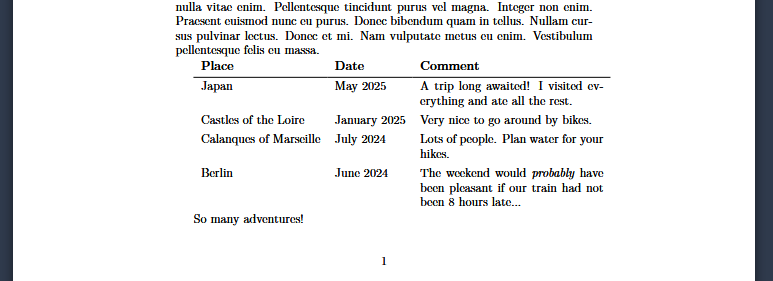
\includegraphics[width=\linewidth]{../img/longtblr_intro}
\end{center}

What if we add a new entry?

\begin{Code}
	Lorem ipsum dolor sit amet.
	% So much more text
	Here's the list of my previous trips:
	
	\begin{tblr}{
		colspec = {llX},
		row{1} = {font=\bfseries},
	}
		Place & Date & Comment \\ \hline
		Japan & May 2025 & A trip long awaited! I visited everything and ate all the rest. \\
		Castles of the Loire & January 2025 & Very nice to go around by bikes. \\
		Calanques of Marseille & July 2024 & Lots of people. Plan water for your hikes. \\
		Berlin & June 2024 & The weekend would \textit{probably} have been pleasant if our train had not been 8 hours late...\\
		Halles Bocuse & April 2014 & Luckily I don't live in Lyon, I would end up overweight and ruined in a matter of days.
	\end{tblr}
	
	So many adventures!
\end{Code}


\begin{center}
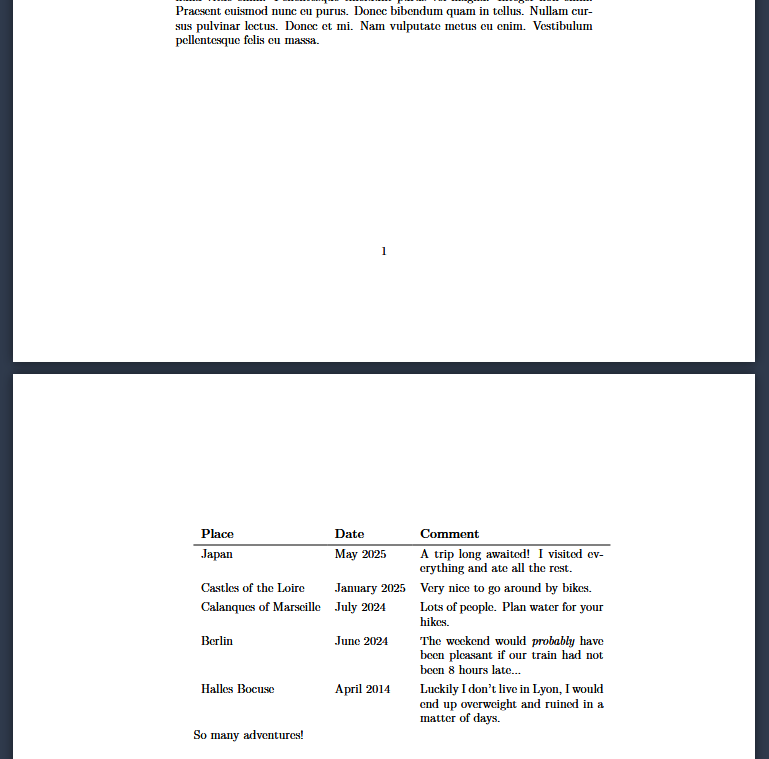
\includegraphics[width=\linewidth]{../img/longtblr_intro2}
\end{center}

Because there is not enough place on the initial page anymore, the table is displayed on the next page and an ugly empty space remains. 

For this reason, it is often better to let Latex decide where the table should be displayed. For this, we signal to Latex to remove the table from the flow of text by passing it to \emph{float mode}. We can also use this as an opportunity to give a caption to our table and a name, that we'll use whenever we want to refer to it.

\begin{Code}
You'll find in Table~\highLight{\ref{table:my-trips}} the list of my previous trips:

\highLight{\begin{table}[htbp]}
	\begin{tblr}{
		colspec = {llX},
		row{1} = {font=\bfseries},
	}
		Place & Date & Comment \\ \hline
	Japan & May 2025 & A trip long awaited! I visited everything and ate all the rest. \\
	Castles of the Loire & January 2025 & Very nice to go around by bikes. \\
	Calanques of Marseille & July 2024 & Lots of people. Plan water for your hikes. \\
	Berlin & June 2024 & The weekend would \textit{probably} have been pleasant if our train had not been 8 hours late...\\
	Halles Bocuse & April 2014 & Luckily I don't live in Lyon, I would end up overweight and ruined in a matter of days.
	\end{tblr}
	\highLight{\caption{All my trips over the last years}\label{table:my-trips}}
\highLight{\end{table}}

So many adventures!
\end{Code}

A few notes:

\begin{itemize}
	\item The environment \snippet{\textbackslash begin\{table\}} and \snippet{\textbackslash end\{table\}} define a floating table. This environment is native from Latex, and does not come from tabularray.
	\item The options \snippet{[htbp]} given to that environment indicate where you would like the table to be, from best desirable outcome to least. Latex will try to make you happy but is sometimes very stubborn about where a table should be. The options stand for:
	\begin{itemize}
		\item \textbf{h}ere: the table is placed where we wrote it in the flow
		\item \textbf{t}op: the table is placed at the top of the current page
		\item \textbf{b}ottom: the table is placed at the bottom of the current page
		\item next \textbf{p}age: the table is placed in the next page.
	\end{itemize}
	\item We added a visible caption with the command \snippet{\textbackslash caption}
	\item We gave a name to the table with the command \snippet{\textbackslash label}, and referred to it with the command \snippet{\textbackslash ref} (you can also use \snippet{\textbackslash cref} if you use the package \snippet{cleveref})
\end{itemize}

\begin{infobox}{TL;DR}
	\begin{itemize}
		\item Use the environment \snippet{\textbackslash begin[htpb]\{table\}} and \snippet{\textbackslash end\{table\}} to transform your table into a float. You can position the float with the options \snippet{h} (here), \snippet{t} (top), \snippet{b} (bottom), \snippet{p} (next page).
		\item Use \snippet{\textbackslash caption} to give a caption to your table, and \snippet{\textbackslash label} to give it a name you can refer to with \snippet{\textbackslash caption}
	\end{itemize}
\end{infobox}
\chapter{Multipage tables}\label{sec:multipage}

Let us now focus to very long tables. All the tables we saw until now could easily fit in a single page, even though that sometimes meant that Latex would move the table to the next page. 

But sometimes, our tables are really too long even for a full page. It is then necessary to split your table on several pages, and tabularray has a command just for that, namely the environment \snippet{longtblr}.

\begin{Code}
\begin{longtblr}{
	colspec={ll},
	row{1} = {font=\bfseries},
}
	Country & Capital \\ \hline
	Afghanistan & Kabul \\
	Albania & Tirana \\
	Algeria & Algiers \\
	Andorra & Andorra la vella
	Angola & Luanda \\
	Antigua and Barbuda & Saint John's \\
	% ... 
	Yemen & Sanaa \\
	Zambia & Lusaka \\
	Zimbabwe & Harare
\end{longtblr}
\end{Code}

I include screenshots of the beginning and end of the first page, of any page in the middle, and the end of the last page:

\begin{center}

\includegraphics[width=\linewidth]{../img/raw_head}


\includegraphics[width=\linewidth]{../img/raw_bottom}


\includegraphics[width=\linewidth]{../img/raw_continued}

%
\includegraphics[width=\linewidth]{img/raw_continued_bottom}


\includegraphics[width=\linewidth]{../img/raw_end}

\end{center}

You can see that the table is automatically horizontally centered, with an empty caption. Some text is also automatically added at the bottom of the page (\textit{Continued on next page}), and the beginning of the following pages (\textit{Continued}).

All these details can be modified. You can also decide of how many rows will be systematically displayed at the top or the bottom of every page. Of how to display the caption. Of many other things still, but these are the main ones. These choices must be declared as an option to \snippet{longtblr}. Other choices must be defined in what tabularray calls templates. It is not very practical but it is how it is.

\begin{Code}

\highLight{\DeclareTblrTemplate{contfoot-text}{default}{(The table continues on the next page)}} 
\highLight{\DeclareTblrTemplate{conthead-text}{default}{(Continued from the previous page)}}

\begin{longtblr}[
	\highLight{caption={All countries and their capital(s)},}
	\highLight{label={table:all_countries},}
]{
	colspec={ll},
	\highLight{rowhead=1,}  % First row will be displayed on every page of the table
	\highLight{rowfoot=1,}  % Last row will be displayed on every page too
	row{odd}= {gray!30},
	row{1} = {font=\bfseries, blue!30},  % appears on every page with rowhead
	row{Z} = {font=\itshape, blue!30},
}
	Country & Capital \\ \hline
	Afghanistan & Kabul \\
	Albania & Tirana \\
	Algeria & Algiers \\
	% ... 
	Yemen & Sanaa \\
	Zambia & Lusaka \\
	Zimbabwe & Harare \\
	\highLight{Country & Capital \\ \hline}  % Repeated on every page thanks to rowfoot
\end{longtblr}
\end{Code}

\begin{center}
	
\includegraphics[width=\linewidth]{../img/pretty_head}
	
	
\includegraphics[width=\linewidth]{../img/pretty_bottom}
	
	
\includegraphics[width=\linewidth]{../img/pretty_continued}
	
%	
\includegraphics[width=\linewidth]{../img/pretty_continued_bottom}
	
	
\includegraphics[width=\linewidth]{../img/pretty_end}
	
\end{center}

\begin{warningbox}{longtblr and compilation time}
	\snippet{longtblr} are quite slow to compile. If your document takes time to compile, look if you can use an alternative such as \snippet{longtable}. Do not use \snippet{longtblr} instead of \snippet{tblr} if your table fits in one page!
\end{warningbox}

One last thing: as we saw, long tables are, by default, horizontally centered. If for any reason you would like to change that, you can use the exterior attribute \snippet{halign}, which can be equal to \snippet{l}, \snippet{c}, \snippet{r}. This is not mentioned anywhere in tabularray documentation but it's always good to know \emoji{slightly-smiling-face}.

\begin{Code}
\begin{longtblr}[
	\highLight{halign=l,}
	caption={All countries and their capital(s)},
	label={table:all_countries},
	]{
		colspec={ll},
		rowhead=1,
		rowfoot=1,
		row{odd}= {gray9},
		row{1} = {font=\bfseries, blue9},
		row{Z} = {font=\itshape, blue9},
	}
	Country & Capital \\ \hline
	Afghanistan & Kabul \\
	Albania & Tirana \\
	% ...
\end{Code}

\begin{infobox}{TL;DR}
	\begin{itemize}
		\item Use \snippet{longtblr} environment for multipage tables
		\item You can specify ``glued'' first and last rows of a longtblr with \snippet{rowhead} and \snippet{rowfoot}, they will appear on every page (for instance, \snippet{rowhead=2})
		\item In option of the \snippet{longtblr} environment, you can give a caption with \snippet{caption=\{...\}}, a name with \snippet{label=\{...\}}, horizontal alignment with \snippet{halign=l} (or \snippet{c}, \snippet{r})
		\item Using templates, you can chose other options, such as personalization of continuation texts with \snippet{\textbackslash DeclareTblrTemplate\{contfoot-text\}\{my-foot\}\{continuation text\} \textbackslash SetTblrTemplate\{contfoot-text\}\{my-foot\}}, same for \snippet{conthead-text}.
	\end{itemize}

No exercise for this chapter because I don't want to make you code long multipage tables \emoji{grinning}.
\end{infobox}
\chapter{Some tabularray libraries}\label{sec:libraries}

We will now explore some very useful functionalities of tabularray, that are relegated to libraries: the ability to draw on your table using tikz, and the ability to have diagonal separations in a cell.

\section{Drawing in your table with Tikz}
\begin{warningbox}{Minimal tabularray version}
The tikz library is only available from tabularray version 2025A or more recent. If the examples in this chapter do not compile for you, check that your version is up to date (there is a guide in \Cref{app:version}).
\end{warningbox}

In order to use tikz\footnote{tikz is a very powerful drawing package for Latex. This document is not a Tikz tutorial, you can some some tutorials at \url{https://tikz.dev/} or \url{https://www.overleaf.com/learn/latex/LaTeX_Graphics_using_TikZ\%3A_A_Tutorial_for_Beginners_(Part_1)\%E2\%80\%94Basic_Drawing}.} in our tables, we will add \snippet{\textbackslash UseTblrLibrary\{tikz\}} in our preamble:

\begin{Code}
\documentclass{article}
\usepackage{tabularray}
\UseTblrLibrary{tikz}  % \Use with uppercase U!

\begin{document}
% Our tables here
\end{document}
\end{Code}

We now can add drawings, either above our table, or below our table:

\begin{Code}
\begin{tblrtikzbelow}
	% Drawings here will be drawn below the table 
\end{tblrtikzbelow}

\begin{tblrtikzabove}
	% Drawings here will be drawn above the table
\end{tblrtikzabove}

\begin{tblr}{}
\end{tblr}
\end{Code}

Note that the environments \snippet{tblrtikzbelow} and \snippet{tblrtikzabove} must be declared before the table where you want to draw.

Moreover, each table cell has coordinates that can be used within tikz drawings. For instance, the cell at the 1st row and 5th coordinate is matched by a tikz node named \snippet{(1-5)}. In general, a node of name \snippet{(i-j)} is matching the cell of coordinates \snippet{(i,j)}. There is also the tikz node \snippet{table}, that encompasses the whole table.

You are now free to use any tikz command and make your table prettier. This tutorial is not a tikz tutorial, so I will simply give a few examples of what can be done. 

The first example is a slight modification of an example from the official tabularray documentation. See how the red lines are drawn above the text, while blue background is drawn below.

\begin{Code}[show-output]
% \usepackage{ninecolors} and \UseTblrLibrary{tikz} in the preamble
\begin{tblrtikzbelow}
	\path[fill=blue!15,draw=blue!80, ultra thick, rounded corners]
	  (table.north west) rectangle (table.south east);
\end{tblrtikzbelow}

\begin{tblrtikzabove}
	\draw[red!70, thick]
	  (2-2.north west) -- (2-3.south east)  % Line from 2-2 top left to 2-3 bottom right
	  (2-2.south west) -- (2-3.north east);  % From 2-2 bottom left to 2-3 top right
\end{tblrtikzabove}

\begin{tblr}{c|c|c|c}
	1-1 & 1-2       & 1-3        & 1-4 \\ \hline
	2-1 & some text & other text & 2-4 \\ \hline
	3-1 & 3-2       & 3-3        & 3-4
\end{tblr}
\end{Code}

Similarly, each intersection \snippet{i,j} (i-th horizontal line and j-th vertical line) has its own name, labelled \snippet{(hi-|vj)}. It can be used as illustrated by the example from the official documentation below:

\begin{Code}[show-output]
\begin{tblrtikzabove}
	\draw[color=green,thick]
	  (h1-|v1) -- (h1-|v2) -- (h2-|v2) -- (h2-|v3) -- (h3-|v3) -- (h3-|v4)
	  -- (h4-|v4) -- (h4-|v5) -- (h2-|v5) -- (h2-|v6) -- (h1-|v6);
\end{tblrtikzabove}

\begin{tblr}{colspec={ccccc},hlines={4pt},vlines={3pt}}
	1-1 & 1-2 & 1-3 & 1-4 & 1-5 \\
	2-1 & 2-2 & 2-3 & 2-4 & 2-5 \\
	3-1 & 3-2 & 3-3 & 3-4 & 3-5
\end{tblr}	
\end{Code}

Incorporating tikz in your tables in quite niche. But when you do need it, it is oh so useful! 
Here is a concrete example, albeit a little bit complicate if you are not familiar with tikz:

% cheating a bit  
\begin{adjustwidth}{-1cm}{-1cm}
\begin{Code}[show-output]
% \usepackage{xcolor}  % in the preamble
% \UseTblrLibrary{tikz}  % in the preamble

\begin{tblrtikzbelow}
	% We draw a rectangle in each cell, between the south west (bottom left);
	% and a mix between north west (top left) and north east (top right), weigthed by
	%  a/b with "a" the value in the cell and "b" the maximum value 9692642
	\draw [white,line width=0.5pt,fill=cyan!20] 
		(2-5.south west) rectangle ($(2-5.north west)!\fpeval{9692642 / 9692642}!(2-5.north east)$)
		(3-5.south west) rectangle ($(3-5.north west)!\fpeval{7809608 / 9692642}!(3-5.north east)$)
		(4-5.south west) rectangle ($(4-5.north west)!\fpeval{7266118 / 9692642}!(4-5.north east)$)
		(5-5.south west) rectangle ($(5-5.north west)!\fpeval{6140419 / 9692642}!(5-5.north east)$)
		(6-5.south west) rectangle ($(6-5.north west)!\fpeval{5424137 / 9692642}!(6-5.north east)$)
		(7-5.south west) rectangle ($(7-5.north west)!\fpeval{5257941 / 9692642}!(7-5.north east)$)
		(8-5.south west) rectangle ($(8-5.north west)!\fpeval{5217075 / 9692642}!(8-5.north east)$)
		(9-5.south west) rectangle ($(9-5.north west)!\fpeval{4085708 / 9692642}!(9-5.north east)$);
	% Don't forget the ; at the end or tikz will crash!
	
	% This can be automrated using the tabularray library "functional"
	% and not having to copy-paste numbers anymore, but this is more complex to do!
	% Such example is implemented in Appendix B 
\end{tblrtikzbelow}

% Original design and table from  https://www.storytellingwithdata.com/blog/2012/02/grables-and-taphs
\begin{tblr}{
	colspec={lcccQ[2.5cm]},
	row{1} = {c, m, font=\bfseries, gray9},
}
	Borough & {Trust \\ rank} & {Index \\ rank } & {Number \\ of grants} & Amount approved (£) \\
	Tower Hamlets          & 1  & 3  & 269 & 9692642 \\
	Hackney                & 2  & 2  & 225 & 7809608 \\
	Southwark              & 3  & 12 & 232 & 7266118 \\
	Camden                 & 4  & 14 & 136 & 6140419 \\
	Islington              & 5  & 4  & 156 & 5424137 \\
	Lambeth                & 6  & 8  & 156 & 5257941 \\
	Newham                 & 7  & 2  & 154 & 5217075 \\
	Hammersmith and Fulham & 8  & 13 & 109 & 4085708 \\
\end{tblr}
\end{Code}
\end{adjustwidth}

You will notice how the tikz code is completely separated from the rest of the table, leaving the data very easy to read and separated from the styling.

\begin{warningbox}{}
tabularray's tikz library is \emph{experimental}: it might or might not evolve in future versions with possible compatibility breaks, even though nothing of the sort is currently planned.
\end{warningbox}

\section{Diagonal separations with diagbox}

Let us finish this tutorial with a very short section, you already suffered more than enough \emoji{grinning}.

By adding \snippet{\textbackslash UseTblrLibrary\{diagbox\}} in the preamble, you can add diagonal separations in a cell, using the commands \snippet{\textbackslash diagbox\{text 1\}\{text 2\}} or \snippet{\textbackslash diagboxthree\{text 1\}\{text 2\}\{text 3\}}.

\begin{Code}[show-output]
% \UseTblrLibrary{diagbox}  % in the preamble

\begin{tblr}{
	colspec={c|ccc},
}
	\diagbox{Day}{Roommate} & Martin & Emma & Julie\\ \hline
	Monday & Dishes & & Cooking\\
	Tuesday & Cooking & Dishes & \\
	Wednesday & & Cooking & Dishes \\
	Thursday & Dishes & & Cooking \\ 
	Friday & Cooking & Dishes & \\
	Saturday & & Cooking & Dishes \\
	Sunday & & & \\
\end{tblr}
\end{Code}

\begin{infobox}{TL;DR}
tabularray offers some libraries with extra functionalities, they can be loaded with \snippet{\textbackslash UseTblrLibrary\{the\_library\_name\}} in the preamble. Among these libraries:

\begin{itemize}
	\item The library \snippet{tikz}, which allows to draw on top (with the environment \snippet{tblrtikzabove}) or below (with the environment \snippet{tblrtikzbelow}) your table. Each cell is given a tikz node named \snippet{(i-j)} and each intersection is given a tikz node named \snippet{(hi-|vj)}.
	\item The library \snippet{diagbox} allows to create cells with a diagonal separator, with \snippet{\textbackslash diagbox\{text 1\}\{text 2\}} or \snippet{\textbackslash diagboxthree\{text 1\}\{text 2\}\{text 3\}}.
\end{itemize}

\textbf{\underline{Exercise:}} recreate the table below.

\begin{center}
	\begin{standalonebox}
% \usetikzlibrary{fadings}  % in the preamble
% \UseTblrLibrary{diagbox}  % in the preamble

\begin{tblrtikzabove}
	\draw [red!80!white, line width=5pt, ->, path fading=east,
	postaction={draw, green!80!white, path fading=west}]
	(2-2.center) -- (2-10.center);
	
	\draw [red!80!white, line width=5pt, ->, path fading=east,
	postaction={draw, green!80!white, path fading=west}]
	(3-3.center) -- (3-12.center);
	
	\draw [red!80!white, line width=5pt, ->, path fading=east,
	postaction={draw, green!80!white, path fading=west}]
	(4-3.center) -- (4-7.center);
	
	\draw [red!80!white, line width=5pt, ->, path fading=east,
	postaction={draw, green!80!white, path fading=west}]
	(5-5.center) -- (5-12.center);
	
	\draw [red!80!white, line width=5pt, ->, path fading=east,
	postaction={draw, green!80!white, path fading=west}]
	(6-3.center) -- (6-10.center);
\end{tblrtikzabove}

\begin{tblr}{
	colspec={r|ccccccccccc},
	colsep={4pt},
	rows={15pt},
}
	\diagboxthree{Country}{Postquantum \\ migration}{Year} & 2025 & 2026 & 2027 & 2028 & 2029 & 2030 & 2031 & 2032 & 2033 & 2034 & 2035 \\ \hline
	Australia &&&&&&&&&&&\\ % 2026-2030 
	ENISA (EU) &&&&&&&&&&&\\ % 2026-2035
	India &&&&&&&&&&&\\ % 2026-2033
	NSA (USA)  &&&&&&&&&&&\\ % 2025-2033	
	United Kingdom &&&&&&&&&&&\\ % 2028-2035
\end{tblr}
	\end{standalonebox}
\end{center}

In order to draw such arrows from node \snippet{(XXX)} to node \snippet{(YYY)}, you can use the command \snippet{\textbackslash draw [red!80!white, line width=5pt, ->, path fading=east, postaction=\{draw, green!80!white, path fading=west\}] (XXX.center) -- (YYY.center);}. You will have to add \snippet{\textbackslash usetikzlibrary\{fadings\}} in the preamble.

In order to make your table prettier, make it so your rows are at least \snippet{12pt} high, and columns have a \snippet{4pt} separation.

The solution is given in \Cref{app:libraries_solution}.
\end{infobox}


You have finished this tutorial. Congratulations \emoji{tada}! 

One last word, we said in the introduction that it was always possible to make tables in native Latex, without the tabularray package. You will find on the next page a quick comparison between the two solutions, slightly modified from \url{https://tex.stackexchange.com/a/760558/430417}

You will also find below some appendix, that contain some helpers to check your tabularray version, a FAQ and some extra crunchy details about tabularray, and the solution to the exercises.

\begin{standalonebox}
\begin{tblr}{
		width={\linewidth},
		colspec={*{3}{X[l]}},
		row{1}={c},
		vlines = {2-Z}{},
		hlines,
		hline{1} = {0pt},
	}
	Feature&\texttt{tabularray}&Traditional \texttt{tabular}s\\
	Complex column specifications. For example, a fixed-width centered column&\SetCell{green!30} Easy. For example, \texttt{Q[c,3cm]}&\SetCell{yellow!30} Not so easy for a newbie. For example, \texttt{>\{\textbackslash centering \textbackslash arraybackslash\}p\{3cm\}}\\
	Row vertical alignment&\SetCell{green!30} Easy with \texttt{valign}: \texttt{t} (top), \texttt{m} (middle), \texttt{b} (bottom), \texttt{h} (head) or \texttt{f} (foot)&\SetCell{red!30} A nightmare\\
	Fixed row height &\SetCell{green!30} Easily customizable with \texttt{ht}&\SetCell{red!30} A nightmare\\
	Vertical space above/below the rows &\SetCell{green!30} Easily customizable with \texttt{rowsep}/\texttt{abovesep}/\texttt{belowsep}&\SetCell{yellow!30} Difficult. You have to redefine \texttt{\textbackslash arraystretch} or set \texttt{\textbackslash extrarowheight} \\
	Cell text with a new line at a desired position (for columns without a fixed width)&\SetCell{green!30} Perfect. Just use \texttt{\{...\textbackslash\textbackslash...\}}&\SetCell{green!30} No problem, but you need \texttt{makecell}\\
	Colored rows with \texttt{booktabs}&\SetCell{green!30} Perfect. No gaps left&\SetCell{red!30} Horrible. White gaps between rules and rows\\
	Multirow text vertical centering&\SetCell{green!30} Easy, including the spanning of the non-multirow rows&\SetCell{red!30} A nightmare. You need a manual adjustment if some of the non-multirow rows are more than one line\\
	Automating. For example, text file (\texttt{.csv}) processing with \texttt{csvsimple-l3}& \SetCell{green!30} Easy because it's possible to totally separate the styles and the contents of the table& \SetCell{yellow!30} Sometimes you need to modify your input. For example, if you need a multirow\\
	Draw pictures above or below your table& \SetCell{green!30} Easy with \texttt{tikz} library&
	\SetCell{yellow!30} More complex. You need to fine-tune the positions \\
	Speed& \SetCell{red!30} Slow &	\SetCell{green!30} No problems \\
	PDF tagging& \SetCell{red!30} Not supported&
	\SetCell{green!30} Supported \\
	Journals/University acceptings& \SetCell{yellow!30} Since it is a relatively new package, some journals or university rules could not accept it&
	\SetCell{green!30} Generally, no problems \\
\end{tblr}
\end{standalonebox}


\appendix
\crefalias{chapter}{appendix}
\crefalias{Chapter}{Appendix}
\crefalias{section}{appendix}
\crefalias{Section}{Appendix}

\chapter{Check your latex version}\label{app:version}

tabularray is a recent package (2021), and might not be present in your installation if it is a bit old. Moreover, package managers who favour stability over new fancy stuff might not ship the latest versions. For instance, at the time of writing of this document Debian bookworm only offers TexLive2022, and thus only the oldest versions of tabularray.

\section{I use TeXLive, but which version?}
You can check your TeXLive version with the command \snippet{tlmgr --version}, which should return something of the like:

\begin{verbatim}
tlmgr --version
# tlmgr revision 76773 (2025-11-06 20:43:29 +0100)
# tlmgr using installation: /usr/local/texlive/2025
# TeX Live (https://tug.org/texlive) version 2025
\end{verbatim}

Which, in this case, means that you are using TeXLive 2025.

In order to update your TeXLive version, use the command \snippet{tlmgr update --all}. With MacOS, you should have a graphical interface with the tool \snippet{Tex Live Utility}.

\section{I am using MikTeX, but which version?}

MikTeX versions matter much less, because you can always update the current one. For instance, after launching the MikTeX console, in the folder \snippet{Updates}, then \snippet{Check for Updates}, you can update your distribution, as well as your tabularray version.

\section{I use Overleaf, how does it work?}

Overleaf uses TeXLive. To change your TeXLive distribution, click on the \snippet{Settings} icon at the bottom left of your workspace, then \snippet{Compiler}, and chose the version you want.

\section{I think that my Latex version is up-to-date, how can I check my tabularray version?}

Either with your Latex package manager (for instance MikTex allows you to right-click on the package, then click ``infos''), either by compiling the following document:

\begin{Code}
\documentclass{article}
\usepackage{tabularray}

\listfiles

\begin{document}
	non-empty document
\end{document}	
\end{Code}

In the compilation logs (a file that ends in \snippet{.log}, or, in Overleaf, by clicking on \snippet{Raw logs}), you will see a lot of text, and at the end of the file, something that looks like 

\begin{verbatim}
{C:/Users/You/AppData/Local/MiKTeX/fonts/map/pdftex/pdftex.map}] (document.aux)
***********
LaTeX2e <2026-06-01>
L3 programming layer <2026-05-26>
***********


*File List*
article.cls    2025/01/22 v1.4n Standard LaTeX document class
size10.clo    2025/01/22 v1.4n Standard LaTeX file (size option)
tabularray.sty    2025-11-27 v2025C Typeset tabulars and arrays with LaTeX3
l3backend-pdftex.def    2026-02-18 L3 backend support: PDF output (pdfTeX)
***********

)
\end{verbatim}

Which allows you to conclude that, in this case, you have tabularray installed in version 2025C.
\chapter{Library functional}\label{app:functional}

The \snippet{functional} library from tabularray is very powerful. It can modify cell contents, their style, etc., before the table is displayed. However, it relies on the \snippet{functional} package, which itself is a modification of the Latex3 syntax, and thus not the most beginner friendly. Nevertheless, after a few dark magic incantations, the results can be stunning. 

Here is an example, that automates the tikz drawing of the table from \Cref{sec:libraries}. Do not panic if you do not understand the code, just remember that the library exists \emoji{slightly-smiling-face}. 

Our preamble gets some weird voodoo:

\begin{Code}
\documentclass{article}  % Or any other documentclass
\usepackage{tabularray}
\UseTblrLibrary{functional, tikz}
\usepackage{xcolor}

% Inspired from https://tex.stackexchange.com/a/750321/430417
\IgnoreSpacesOn
% Variable must be def before the function
\tlNew \gTikzPercentagePathsTl

% Computes a column's maximum.
% Useful if numbers are not ordered.
\prgNewFunction \colMaxValue {m} {  % takes a mandatory argument, #1, the column where we want to compute the max
	\fpSet \lTmpaFp {\fpEval {\cellGetText{2}{#1}}}  % saving temp max in \lTmpaFp 
	\intStepOneInline {2} {\arabic{rowcount}} {  % ##1 starts from 2 until the number of rows
		\fpSet \lTmpaFp {\fpMathMax{\lTmpaFp}{\fpEval {\cellGetText{##1}{#1}}}}  % update temp max
	}
	\prgReturn {\fpUse\lTmpaFp}
}

\prgNewFunction \barPlotPaths {m} {  % #1 is the index of the column we want the bars
	\tlClear \gTikzPercentagePathsTl  % set the var in which we will store the drawing instructions
	\fpSet \lTmpaFp {\colMaxValue{#1}}  % Set #1 column max value in \lTmpaFp
	\intStepOneInline {2} {\arabic{rowcount}} {  % ##1 starts from 2 until max row
		\fpSet \lTmpbFp {\fpEval{\cellGetText{##1}{#1}}}  % save cell (##1, #1) value into \lTmpbFp 
		\fpSet \lTmpcFp {\fpMathDiv {\lTmpbFp} {\lTmpaFp}}  % save (cell value) / (max value) in \lTmpcFp
		\tlPutRight \gTikzPercentagePathsTl {  % Update drawing instruction with a rectangle of size \lTmpcFp
			\evalWhole{
				(##1-#1.south~west) rectangle
				($(##1-#1.north~west)!{\fpUse \lTmpcFp}!(##1-#1.north~east)$)
			}
		}
	}
}
\IgnoreSpacesOff
\end{Code}

So that our table does not require any copy pasting anymore!

\begin{Code}[show-output]
\begin{tblrtikzbelow}
	% draw everything from \gTikzPercentagePathsTl
	\highLight{\draw[white, line width=0.5pt, fill=cyan!20] \gTikzPercentagePathsTl;}
\end{tblrtikzbelow}

% Original table and design from https://www.storytellingwithdata.com/blog/2012/02/grables-and-taphs
\begin{tblr}{
	colspec={lcccQ[2.5cm]},
	row{1} = {c, m, font=\bfseries, gray9},
	\highLight{process={\barPlotPaths{5}},}  % We call the function barPlotPath defined in the preamble to fill \gTikzPercentagePathsTl with bars to plot in the 5th column
}
	Borough & {Trust \\ rank} & {Index \\ rank } & {Number \\ of grants} & Amount approved (£) \\
	% no more data copy-pasting!
	Tower Hamlets          & 1  & 3  & 269 & 9692642 \\
	Hackney                & 2  & 2  & 225 & 7809608 \\
	Southwark              & 3  & 12 & 232 & 7266118 \\
	Camden                 & 4  & 14 & 136 & 6140419 \\
	Islington              & 5  & 4  & 156 & 5424137 \\
	Lambeth                & 6  & 8  & 156 & 5257941 \\
	Newham                 & 7  & 2  & 154 & 5217075 \\
	Hammersmith and Fulham & 8  & 13 & 109 & 4085708 \\
\end{tblr}
\end{Code}

\chapter{Advanced colspec}\label{app:colspec}

In this tutorial, we saw that \snippet{colspec} could contain information on the colunms and vertical borders of your table. But, just like with native Latex tables, there is more to it. In most cases however, tabularray has a header option that is preferrable.

\section{Column separation}

The directive \snippet{@\{\}} allows to specify what Latex must insert between two columns. For instance, if you want two columns to be separated by \snippet{2cm}, you can write:

\begin{Code}[show-output]
\begin{tblr}{
	colspec={l\highLight{@{\hspace{2cm}}}cr},
}
	a & b & c
\end{tblr}
\end{Code}

It is often better to rather use the \snippet{colsep} (margin on both sides), \snippet{leftsep}, \snippet{rightsep} options from tabularray, as they have the advantage of not being completely counter-intuitive: the \snippet{@\{\}} is incompatible with a vertical border, and the extra space does not belong to any column, therefore cannot be styled:

\begin{Code}[show-output]
\begin{tblr}{
	colspec={l@{\hspace{2cm}}c@{\hspace{2cm}}r},
	column{1} = {green!20},
	column{2} = {red!20},
	column{3} = {blue!20},
	vline{2}, % will break spacing between the first two columns
}
	a & b & c
\end{tblr}	
\end{Code}

\begin{Code}[show-output]
\begin{tblr}{
	colspec={lcr},
	column{1} = {rightsep=1cm, green!20},
	column{2} = {colsep=1cm, red!20},
	column{3} = {leftsep=1cm, blue!20},
	vline{2} = {},  % does not break anything
}
	a & b & c
\end{tblr}
\end{Code}

\section{Text at the beginning and the end of a cell}

Let us mention the operators \snippet{>\{\}} and \snippet{<\{\}}, who respectively add some text at the beginning and at the end of each cell of the column. Rather than long explanations, here is an example: 

\begin{Code}[show-output]
\begin{tblr}{\highLight{>{Candidate }}ccc\highLight{<{s}}}
      & Name   & Time in~\\ \hline
	1 & Claude & 10.5 \\
	2 & Mary   & 5.68 \\
	3 & Jorgen & 12.8 \\
\end{tblr}
\end{Code}

Here again, tabularray has the options \snippet{preto} and \snippet{appto} that are preferrable and do same thing in most cases. If you want to add commands with the operators  \snippet{>} and \snippet{<}, you will maybe have to use the option \snippet{cmd} instead. I will let you refer to the documentation for this one.

\section{Several times the same column}

When our table has numerous columns, writing dozens of times the same instruction in the colspec can quickly become repetitive. Luckily, you can replace this by, for instance, \snippet{*\{3\}\{c|Q[l,2cm]\}}, which is the same thing as \snippet{c|Q[l,2cm]c|Q[l,2cm]c|Q[l,2cm]}.
Here is an example, with as a bonus a use of the option \snippet{cmd} that we talked about just above.

\begin{Code}
\documentclass{standalone}
\usepackage{tabularray, xcolor, ninecolors}
\usepackage{adjustbox}  % for \adjustbox that rotates a textbox
\usepackage{bbding}  % for \Checkmark and \XSolidBrush
\newcommand{\yes}{\textcolor{green!70!black}{\Checkmark}}
\newcommand{\no}{\textcolor{red!50}{\XSolidBrush}}

\begin{document}
\begin{tblr}{
	colspec={Q[2cm,r,m]\highLight{*{27}{c}}},  % One 2cm column, and 27 centered ones
	columns = {font={\small},colsep=3.5pt},
	row{1} = {cmd=\adjustbox{angle=45,lap=\width-(1em)}},
	% the cmd option applies the command adjustbox (rotation) to every cell in the first row
}
	& Austria & Belgium & Bulgaria & Croatia & Cyprus & Czechia & Denmark & Estonia & Finland & France & Germany & Greece & Hungary & Ireland & Italy & Latvia & Lithuania & Luxembourg & Malta & Netherlands & Poland & Portugal & Romania & Slovakia & Slovenia & Spain & Sweden
	Eurozone & \yes & \yes & \yes & \yes & \yes & \yes & \no & \yes & \yes & \yes & \yes & \yes & \no & \yes & \yes & \yes & \yes & \yes & \yes & \yes & \no & \yes & \no & \yes & \yes & \no & \no \\
	Schengen Area & \yes & \yes & \yes & \yes & \no & \yes & \yes & \yes & \yes & \yes & \yes & \yes & \yes & \no & \yes & \yes & \yes & \yes & \yes & \yes & \yes & \yes & \yes & \yes & \yes & \yes & \yes & \\ 
	European Economic Area & \yes & \yes & \yes & \yes & \yes & \yes & \yes & \yes & \yes & \yes & \yes & \yes & \yes & \yes & \yes & \yes & \yes & \yes & \yes & \yes & \yes & \yes & \yes & \yes & \yes & \yes & \yes & \\ 
\end{tblr}
\hspace{2em} % a bit of extra space to avoid cutting the end of our table
\end{document}
\end{Code}

Will give:

\begin{center}
\begin{standalonebox}
\begin{tblr}{
	colspec={Q[2cm,r,m]*{27}{c}},  % One 2cm column, and 27 centered ones
	columns = {font={\small},colsep=3.5pt},
	row{1} = {cmd=\adjustbox{angle=45,lap=\width-(1em)}},
	% the cmd option applies the command adjustbox (rotation) to every cell in the first row
}
	& Austria & Belgium & Bulgaria & Croatia & Cyprus & Czechia & Denmark & Estonia & Finland & France & Germany & Greece & Hungary & Ireland & Italy & Latvia & Lithuania & Luxembourg & Malta & Netherlands & Poland & Portugal & Romania & Slovakia & Slovenia & Spain & Sweden \\
	Eurozone & \yes & \yes & \yes & \yes & \yes & \yes & \no & \yes & \yes & \yes & \yes & \yes & \no & \yes & \yes & \yes & \yes & \yes & \yes & \yes & \no & \yes & \no & \yes & \yes & \no & \no \\
	Schengen Area & \yes & \yes & \yes & \yes & \no & \yes & \yes & \yes & \yes & \yes & \yes & \yes & \yes & \no & \yes & \yes & \yes & \yes & \yes & \yes & \yes & \yes & \yes & \yes & \yes & \yes & \yes & \\ 
	European Economic Area & \yes & \yes & \yes & \yes & \yes & \yes & \yes & \yes & \yes & \yes & \yes & \yes & \yes & \yes & \yes & \yes & \yes & \yes & \yes & \yes & \yes & \yes & \yes & \yes & \yes & \yes & \yes & \\ 
\end{tblr}
\end{standalonebox}
\end{center}

\section{No colspec}

I have to confess something: the colspec option is not mandatory. As a matter of fact, tabularray computes the table structure from the ampersands \snippet{\&} in each row. Moreover, in case of conflict between the colspect and the table body, the table body wins (remember the priority rules!).

\begin{Code}
\begin{tblr}\highLight{{}}  % also works
	Hello & tabularray & world! \\
	cell & other cell & last cell \\
\end{tblr}
\end{Code}

The colspec option is essentially useful to give the reader a quick indication about the table structure, and is also useful for applying basic styling to each column. I strongly encourage you to always write the colspec, but know that if there are not enough columns in the compiled table, it's probably because you forgot a few \snippet{\&} somewhere!

Finally, the colspec is mandatory with native Latex tables, so if one day you have to migrate your tables back to native, you will know what to do.


\chapter{Solution to the exercises}\label{app:solutions}

\section{Solution to \Cref{sec:basic}}\label{app:solution_basic}
\begin{Code}[show-output]
% \usepackage{tabularray} % in the preamble
\begin{tblr}{|l|c|r|}  % 3 columns, and vertical borders everywhere
	\hline
	Hello & tabularray  & world! \\
	cell  & cell & last table cell \\
	\hline
\end{tblr}
\end{Code}


\section{Solution to \Cref{sec:control}}\label{app:solution_control}
\begin{Code}[show-output]
\begin{tblr}{colspec={Q[1.5cm]lXX[2,j]}, width=0.8\linewidth}
	\SetCell[c=2]{c} Region &             & Celebrity                                        & Short bio \\ \hline
	\SetCell[r=3]{m} Europe & Russia      & \SetCell[r=2]{} {Leonhard Euler \\(1707--1783) } & \SetCell[r=2]{}   One of the greatest mathematicians in history, he also made significant contributions to mechanics, fluid dynamics, optics and astronomy.\\  \hline
	empty                   & Switzerland & empty                                            & not displayed either \\ \hline
	& Greece  & {Socrates \\(-470 -- -399)}                          & One of the founders of philosophy. He left no written works; the only record of his thinking comes from his pupils Plato and Xenophon. \\ \hline
	\SetCell[r=2]{} Asia    & Japan       & {Katsushika Hokusai \\(1760--1849)}              & A painter, draughtsman and printmaker, he is world-renowned for his woodblock print \textit{The Great Wave off Kanagawa}. He had a lasting influence not only on Japanese art, but also on European art (Van Gogh, Monet, Degas, etc.) \\ \hline
	& India       & {Suśruta \\ (around -600)}                       & He wrote one of the seminal texts on Ayurvedic medicine and made major discoveries in the fields of cataract surgery and plastic surgery. He is regarded as the father of surgery. \\ \hline
\end{tblr}
\end{Code}

\section{Solution to \Cref{sec:separations}}\label{app:separations_solution}
There are several possible solutions.
\begin{Code}[show-output]
	\begin{tblr}{
			hlines,
			vlines,
			colsep=8pt,
			rowsep=6pt,
			hspan=minimal,
			vspan=even,
			colspec={Q[l,2cm,m]lll}
		}
		Title & Author & Year & \SetCell[r=2]{} Excerpt \\
		\SetCell[c=3]{c} Comment & & & \\
		Les Djinns & Victor Hugo &  1829 & \SetCell[r=2]{m} {Mur, ville,\\ Et port, \\ Asile \\ De mort, \\ Mer grise \\ Où brise \\ La brise, \\Tout dort.} \\
		\SetCell[c=3]{l} A beautiful poem in which each stanza has a different metrical structure. & & & \\
		Colloque sentimental & Paul Verlaine & 1869 & \SetCell[r=2]{m} {Dans le vieux parc solitaire et glacé \\ Deux formes ont tout à l'heure passé. \\[1em] Leurs yeux sont morts et leurs lèvres sont molles, \\ Et l'on entend à peine leurs paroles.} \\
		\SetCell[c=3]{l} A conclusion to the compilation ``Fêtes galantes'' that stands in stark contrast to the rest by its darkness and melancholy. \\
	\end{tblr}
\end{Code}

\section{Solution to \Cref{sec:styling}}\label{app:styling_solution}

Not easy! There are, of course, several solutions.

\begin{Code}[show-output]
\begin{tblr}{
		colspec = {rcccccc},
		%
		% rows
		row{even[4]} = {gray!20},
		row{Z[2],Z} = {white}, % overload to avoid gray in the last 2 rows
		% We could have used row{every[2]{4}{-2}} = {gray!20},
		% (but we did not see this selector in the tutorial)
		row{Z} = {font=\bfseries},
		%
		% cells 
		% merging cells
		cell{1}{even} = {c=2}{c},
		cell{Z}{even} = {c=2}{c},
		% Background colours
		cell{2,Z[2]}{even} = {green!30},
		cell{2,Z[2]}{odd[3]} = {red!20},
		% styling for qualified/disqualified
		cell{qualified} = {green!60!black, fg=white},
		cell{disqualified} = {red!80!black, fg=white},
		%
		% borders
		hline{2} = {2-Z}{dashed},
		hline{3},  % empty style means default style
		hline{Z[3]} = {2pt},
		vline{4,6} = {2-Z}{},
	}
	& Mini &&  Juniors && Seniors &\\
	& Won & Lost & Won & Lost & Won & Lost \\
	Day 1 & 2 & 3 & 5 & 1 & 3 & 4 \\
	Day 2 & 4 & 1 & 2 & 4 & 7 & 0 \\
	Day 3 & 0 & 5 & 3 & 3 & 3 & 4 \\
	Day 4 & 2 & 3 & 1 & 5 & 4 & 3 \\
	Day 5 & 3 & 2 & 5 & 1 & 6 & 1 \\
	Day 6 & 4 & 1 & 3 & 3 & 2 & 5 \\
	Total & 15 & 15 & 19 & 17 & 25 & 17 \\
	Qualified? & \SetChild{class=disqualified}No && \SetChild{class=qualified}Yes && \SetChild{class=qualified}Yes\\
\end{tblr}
\end{Code}

Small tip: remember that you cannot have blank lines in the header. However, you can have lines of comments, to keep some distance between each part of your styling.

For comparison, here is the same styling, but exclusively using in-body styling. As you'll see, it's much less pretty.

\begin{Code}
\begin{tblr}{rcccccc}
& \SetCell[c=2]{} Mini && \SetCell[c=2]{}Juniors && \SetCell[c=2]{} Seniors &\\ \SetHline{2-Z}{dashed}
& \SetCell{green9} Won & \SetCell{red9} Lost & \SetVline{2-Z}{} \SetCell{green9} Won & \SetCell{red9} Lost & \SetVline{2-Z}{} \SetCell{green9} Won & \SetCell{red9} Lost \\ \hline
Day 1 & 2 & 3 & 5 & 1 & 3 & 4 \\
\SetRow{gray9} Day 2 & 4 & 1 & 2 & 4 & 7 & 0 \\
Day 3 & 0 & 5 & 3 & 3 & 3 & 4 \\
\SetRow{gray9} Day 4 & 2 & 3 & 1 & 5 & 4 & 3 \\
Day 5 & 3 & 2 & 5 & 1 & 6 & 1 \\
\SetRow{gray9} Day 6 & 4 & 1 & 3 & 3 & 2 & 5 \\ \hline[2pt]
Total & \SetCell{green9} 15 & \SetCell{red9} 15 & \SetCell{green9} 19 & \SetCell{red9} 17 & \SetCell{green9} 25 & \SetCell{red9} 17 \\
\textbf{Qualified?} & \SetCell[c=2]{red5, fg=white} \textbf{No} && \SetCell[c=2]{green5, fg=white}\textbf{Yes} && \SetCell[c=2]{green5, fg=white} \textbf{Yes}\\
\end{tblr}
\end{Code}

You now understand why it is advised to use header styling as much as possible! If you look at the last two rows, the data are lost in a flood of styling instructions. With this code, good luck for debugging any error...

\section{Solution to \Cref{sec:libraries}}\label{app:libraries_solution}

\begin{Code}[show-output]
% \usepackage{xcolor}  % in the preamble
% \UseTblrLibrary{tikz, diagbox}  % in the preamble
% \usetikzlibrary{fadings}  % in the preamble

\begin{tblrtikzabove}
	\draw [red!80!white, line width=5pt, ->, path fading=east,
	postaction={draw, green!80!white, path fading=west}]
	(2-2.center) -- (2-10.center);
	
	\draw [red!80!white, line width=5pt, ->, path fading=east,
	postaction={draw, green!80!white, path fading=west}]
	(3-3.center) -- (3-12.center);
	
	\draw [red!80!white, line width=5pt, ->, path fading=east,
	postaction={draw, green!80!white, path fading=west}]
	(4-3.center) -- (4-7.center);
	
	\draw [red!80!white, line width=5pt, ->, path fading=east,
	postaction={draw, green!80!white, path fading=west}]
	(5-5.center) -- (5-12.center);
	
	\draw [red!80!white, line width=5pt, ->, path fading=east,
	postaction={draw, green!80!white, path fading=west}]
	(6-3.center) -- (6-10.center);
\end{tblrtikzabove}

\begin{tblr}{
		colspec={r|ccccccccccc},
		rows={15pt},
		colsep={4pt},
	}
	\diagboxthree{Country}{Postquantum \\ migration}{Year} & 2025 & 2026 & 2027 & 2028 & 2029 & 2030 & 2031 & 2032 & 2033 & 2034 & 2035 \\ \hline
	Australia &&&&&&&&&&&\\ % 2026-2030 
	ENISA (EU) &&&&&&&&&&&\\ % 2026-2035
	India &&&&&&&&&&&\\ % 2026-2033
	NSA (USA)  &&&&&&&&&&&\\ % 2025-2033	
	United Kingdom &&&&&&&&&&&\\ % 2028-2035
\end{tblr}
\end{Code}

The drawing code can be simplified if you know a bit of tikz:

\begin{Code}
\begin{tblrtikzabove}
	% We define a reusable style
	\tikzset{
		myarrow/.style={
			red!80!white,
			line width=5pt,
			->,
			path fading=east,
			postaction={draw, green!80!white, path fading=west}
		}
	}
	
	\draw[myarrow] (2-2.center) -- (2-10.center);
	\draw[myarrow] (3-3.center) -- (3-12.center);
	\draw[myarrow] (4-3.center) -- (4-7.center);
	\draw[myarrow] (5-5.center) -- (5-12.center);
	\draw[myarrow] (6-3.center) -- (6-10.center);
\end{tblrtikzabove}
\end{Code}

We could also make it so that the code uses semantic numbers (i.e. draw \snippet{(2.2026.center) -- (2-2030.center)} rather than the current code, and even use the library functional to have the years written in the table, then automatically processed and deleted from the output, but this is left as an exercise to the reader.


\end{document}
